%%%%%%%%%%%%%%%%%%%%%%%%%%%%%%%%%%%%%%%%%%%%%%%%%%%%%%%%%%%%%%%%%%%%%%%%%%%%%
%%%
%%% File: thesis.tex, version 1.8, April 2025
%%%
%%% =============================================
%%% This file contains a template that can be used with the package
%%% cs.sty and LaTeX2e to produce a thesis that meets the requirements
%%% of the Computer Science Department from the Technical University of Cluj-Napoca
%%%%%%%%%%%%%%%%%%%%%%%%%%%%%%%%%%%%%%%%%%%%%%%%%%%%%%%%%%%%%%%%%%%%%%%%%%%%%

\documentclass[12pt,a4paper,twoside]{report}

\usepackage{cs}
\usepackage[T1]{fontenc}
\usepackage[utf8]{inputenc}
\usepackage[english,romanian]{babel}
\usepackage{times}
\\usepackage{graphicx} % Enable images for final version
\usepackage{float} % for [H] exact figure placement
\usepackage{latexsym}
\usepackage{amsmath,amsbsy}
\usepackage{amssymb}
\usepackage[matrix,arrow]{xy}
\usepackage{ae,aecompl}
\usepackage{amstext}
\usepackage{graphics}
\usepackage{ae,aecompl}
% \usepackage{algorithm} % Comment out if not available
\usepackage{color}
\usepackage{titlesec}
\usepackage{fancyhdr}
\usepackage{booktabs}
\usepackage{hyperref}
%% decomentati linia urmatoare pentru e nu mai evidenția hiper legăturile pentru imprimare pe hârtie
%\hypersetup{hidelinks}
\usepackage{geometry}
\usepackage{lipsum}
\usepackage{enumitem}
%\usepackage{microtype}
\usepackage[capitalise,nameinlink]{cleveref}
% Pentru comanda \FloatBarrier inserată în capitolele tehnice
\usepackage{placeins}

% Default graphics paths
% \graphicspath{{figs/}{figs/CAPITOLUL 7/}} (comentat – imagini omise)

% Define colors
\definecolor{BrandBlue}{RGB}{0, 102, 204}
\definecolor{teal}{RGB}{0, 128, 128}

%%%%%%%%%%%%%%%%%%%%%%%%%%%%%%%%%%%%%%%%%%%%%%%%%%%%%%%%%%%%%
\setlist{noitemsep,nolistsep}


\diplomathesis
\centerchapter
\singlespace
\newenvironment{definition}[1][Definiție.]{\begin{trivlist}
\item[\hskip \labelsep {\bfseries #1}]}{\end{trivlist}}

%%% setari pagină
 \geometry{
	a4paper,
	total={159.2mm,246.2mm},
	left=25.4mm,
	top=25.4mm,
}


\begin{document}
%\frontmatter
%%%%%%%%%%% Stil pentru paginile de capăt
\pagestyle{fancy}
\setlength{\voffset}{-10pt}
\setlength\headheight{70.0pt}
%\addtolength{\textheight}{-80.0pt}
\renewcommand{\headrulewidth}{0pt}
\chead{%
	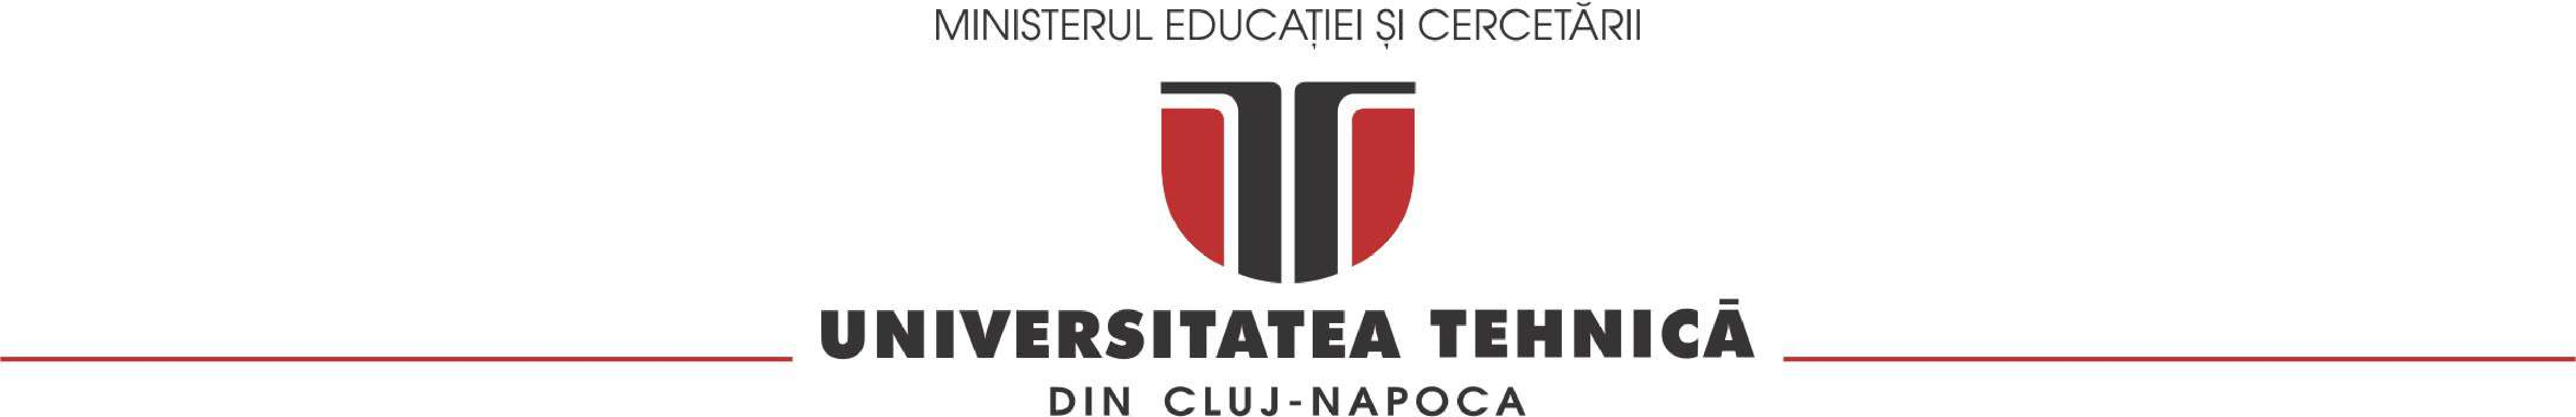
\includegraphics[width=\textwidth]{figs/AntetUTCNRom.pdf}
}
\cfoot{}
\lfoot{}
\rfoot{}
%%%%%%%%%%%%%%%%%%%%%%%%%%%%%% Schimbați corespunzător ultimul element
\renewcommand{\thesisauthor}{Dan Lucian GHILEA}    %% Prenumele și numele dvs.
\renewcommand{\thesismonth}{Septembrie}     %% Luna sesiunii de licență
\renewcommand{\thesisyear}{2025}      %% Anul sesiunii de licență
\renewcommand{\thesistitle}{%
  ArtAdvisor: Proiectarea unui Asistent Conversațional pentru Interpretarea Multi-Modală și Narativă a Artei
  \\[1.5em] % Adaugă un spațiu vertical elegant între titlu și subtitlu
  \large % Setează o dimensiune mai mică pentru fontul subtitlului
  --- O Arhitectură Bazată pe Ansambluri de Deep Learning, Generare de Limbaj și Sinteză Vocală ---
}\renewcommand{\thesissupervisor}{As. dr. ing. Cristina Maria FEIER} %% Conducătorul științific
%%%%%%%%%%%%%%%%%%%%%%%%%%%%%%%%%%%%%
\newcommand{\makeThesisTitle}{\textbf{\thesistitletypesize \thesistitle}}
\newcommand{\makeThesisType}{\thesistypetypesize \thesistype}
\newcommand{\department}{\sffamily\bfseries\small FACULTATEA DE AUTOMATICĂ ȘI CALCULATOARE\\
	DEPARTAMENTUL CALCULATOARE} 
\renewcommand{\thesistype}{LUCRARE DE LICENȚĂ}
\newcommand{\uline}[1]{\rule[0pt]{#1}{0.4pt}}
% Headings pentru folie de capăt
%%%%% Pagina cu titlul tezei nu trebuie să schimbati nimic %%%%%%%%%%%%%%%%%%%%%%%%
\begin{center}
	{\department}
	
	\vspace{4cm}
	\makeThesisTitle
	~\\~\\
	
	\makeThesisType
	
	~\\\vspace{6.5cm}
	
	\begin{tabular}{p{.3\linewidth}p{.5\linewidth}}
		{\hfill Absolvent:} & {\bf \thesisauthor} \\
		&\\
		{\parbox[t]{\linewidth}{\qquad\qquad\qquad Coordonator\\\hspace*{3.2cm}științific:}}& {\bf \thesissupervisor}\\
	\end{tabular}
	
	\vspace{3cm}
	{\bf \thesisyear}
\end{center}
%%%%%%%%%%%%%%%%%%%%%%%%%%%%%%%%%%%%%%%%%%%%%%%%%%%%%
\newpage
%%%%%%% Pagina cu tema %%%%%%%%%%%%%%%%%%%%%%%%%%%%%%%
\begin{center}
	{\department}
\end{center}
\vspace{0.5cm}

%\begin{small}
\begin{tabular}{p{7cm}p{8cm}}
	%\hspace{-1cm}& VIZAT,\\
	\hspace{-1cm}DECAN, & DIRECTOR DEPARTAMENT,\\
	\hspace{-1cm}{\bf Prof. dr. ing. Vlad MUREȘAN} & {\bf Prof. dr. ing. Rodica POTOLEA}\\  
\end{tabular}

\vspace{2cm}

\begin{center}
	Absolvent: {\bf \thesisauthor}
	
	\vspace{1cm}
	
	{\bf \thesistitle}
\end{center}

\vspace{5mm}
%%%%%%%%%%%%%%%%%%%%%%% Aici modificați
\begin{enumerate}
	\item {\bf Enunțul temei:} {\it Scurtă descriere a temei lucrării de licență și datele inițiale}
	\item {\bf Conținutul lucrării:} {\it (enumerarea părților componente) Exemplu: Pagina de prezentare, aprecierile coordonatorului de lucrare, titlul capitolului 1, titlul capitolului 2, titlul capitolului n, bibliografie, anexe.}
	\item {\bf Locul documentării:} {\it Exemplu}: Universitatea Tehnică din Cluj-Napoca, Departamentul Calculatoare
	\item {\bf Consultanți:}
	\item {\bf Data emiterii temei:} 1 Noiembrie 2024 %%%%%%%%%%%%% Modificați corespunzător
	\item {\bf Data predării:} 11 Septembrie 2025 %%%%%%%%%%%%%%% Modificați corespunzător
\end{enumerate}
\vspace{1.2cm}

\hspace{6cm} Absolvent: \uline{6cm} 

\vspace{0.5cm}
\hspace{6cm} Coordonator științific: \uline{5cm} 
\newpage
%%%%%%%%% Pagina cu declarația
\begin{center}
	{\department}
\end{center}
\vspace{0.5cm}

\begin{center}
	{\bf Declarație pe propria răspundere privind\\ 
		autenticitatea lucrării de licență}
\end{center}
\vspace{1cm}

\begin{minipage}{\linewidth}
	\indent Subsemnatul(a) \uline{.73\linewidth},
	\uline{.82\linewidth} %% locul pentru nume prenume
	legitimat(ă) cu\\ \uline{4cm} %% locul pentru tipul documentului de identitate
	seria \uline{3cm} % seria documentului de identitate 
	nr. \uline{6.3cm} % numărul documentului de identitate 
	CNP \uline{9cm}, % CNP
	autorul lucrării\
	\uline{\linewidth} % titlul lucrării
	\uline{\linewidth} % titlul lucrării
	elaborată în vederea susținerii examenului de finalizare a studiilor de licență la Facultatea de Automatică și Calculatoare, Specializarea \uline{7cm} % numele specializării
	din cadrul Universității Tehnice din Cluj-Napoca, sesiunea \uline{4cm} % numele sesiunii de licență (luna)
	 a anului universitar \uline{3cm}, % anul de început al anului universitar
	  declar pe propria răspundere că această lucrare este rezultatul propriei activități intelectuale, pe baza cercetărilor mele și pe baza informațiilor obținute din surse care au fost citate, în textul lucrării și în bibliografie.\\
	\hspace*{8mm} Declar că această lucrare nu conține porțiuni plagiate, iar sursele bibliografice au fost folosite cu respectarea legislației române și a convențiilor internaționale privind drepturile de autor.\\
	\hspace*{8mm} Declar, de asemenea, că această lucrare nu a mai fost prezentată în fața unei alte comisii de examen de licență.\\
	\hspace*{8mm} În cazul constatării ulterioare a unor declarații false, voi suporta sancțiunile administrative, respectiv, \emph{anularea examenului de licență}.
\end{minipage}
\vspace{1.5cm}

Data \hspace{8cm} Nume, Prenume

\vspace{0.5cm}

\uline{3cm} \hspace{5cm} \uline{5cm}

\vspace{1cm}
\hspace{9.4cm}Semnătura
\newpage
 % Primele 3 pagini
%%%%%%%%%%%%%%%%% Pagina cu instructiuni de eliminat
\thispagestyle{empty}
\thispagestyle{empty}
\begin{center}\large
	Instrucțiuni generale.
\end{center}
~\\

{\color{red}\large{\bf De citit înainte} (această pagină se va elimina din versiunea finală)}:\\
\begin{enumerate}
 \item Cele trei pagini anterioare (foaie de capăt, foaie sumar, declarație) se vor lista pe foi separate (nu față-verso), fiind incluse în lucrarea listată.
 Foaia de sumar (a doua) necesită semnătura absolventului, respectiv a coordonatorului.
 Pe declarație se trece data când se predă lucrarea la secretarii de comisie.
 \item Pe foaia de capăt, se va trece corect titulatura cadrului didactic îndrumător, în engleză (consultați pagina de unde ați descărcat acest document pentru lista cadrelor didactice cu titulaturile lor).
 \item Fiecare capitol începe pe pagină nouă.
 \item Marginile paginilor nu se modifică.
 \item Respectați restul instrucțiunilor din fiecare capitol.
 \item Am inclus pachetul \verb+hyperref+ pentru a genera legături de navigare atât în document cât și la link-uri de web. Pentru listarea pe hârtie a fișierului pdf decomentați linia care conține \verb+%\hypersetup{hidelinks}+
 aflată în partea de început a fișierului principal \verb+thesis_rom.tex+.
\end{enumerate}

\newpage
%%%%%%%%%%%%%%%%%% sf. pagina cu instructini
\pagestyle{fancy}
\setlength\headheight{16.0pt}
\renewcommand{\chaptermark}[1]{\markboth{\chaptername~\thechapter.~#1}{}}
\renewcommand{\sectionmark}[1]{\markright{\thesection\ #1}}
\renewcommand{\headrulewidth}{0.4pt}
\lhead{}
\chead{%
	\leftmark\rightmark
}
\chead{}
\cfoot{\thepage}
\lfoot{}
\rfoot{}

%%%%%%%%%%%% Cuprinsul %%%%%%%%%%%%%%%%%%%%%%%%%%%%%%%%%%%%%%%%
\pagenumbering{roman}
\setcounter{page}{1}

\newpage

\tableofcontents

\newpage

%\listoftables
%\listoffigures

%%%%%%%%%%%%%%%%%% de aici începe numerotarea paginilor
\pagenumbering{arabic}
\setcounter{page}{1}


\titleformat{\chapter}[hang]
{\normalfont\Large\bfseries}{\chaptertitlename\ \thechapter.}{1em}{}
\titleformat{\section}[hang]
{\normalfont\large\bfseries}{\thesection.}{1em}{}
\titleformat{\subsection}[hang]
{\normalfont}{\thesubsection.}{1em}{}
\titlespacing*{\section}{0pt}{12pt}{6pt}
\titlespacing*{\subsection}{0pt}{12pt}{6pt}
\titlespacing*{\chapter}{0pt}{30pt}{18pt}

\chapter{Introducere}
\label{ch:introducere}

\section{Contextul proiectului}
\label{sec:intro-context}

Arta picturală a fost dintotdeauna un mediu privilegiat de exprimare a emoțiilor. Prin culoare, lumină, compoziție și textură, artiștii transmit stări nuanțate, adesea simultane, care solicită din partea publicului atât sensibilitate estetică, cât și un minim repertoriu interpretativ. În era accesului digital la patrimoniu, „a vedea" nu înseamnă automat „a înțelege": utilizatorul ajunge ușor la imagine, dar rămâne adesea fără repere afective explicite.

În acest context, proiectele de mediere culturală pot beneficia de contribuția interdisciplinară a informaticii și științelor cognitive. Inteligența artificială aplicată imaginilor, psihologia afectului și designul centrat pe utilizator converg către instrumente capabile să conecteze percepția cu interpretarea. O prezentare afectivă clară, sobră și accesibilă are valoare educațională pentru publicul larg, valoare curatorială pentru organizarea conținutului în medii digitale și valoare de cercetare pentru testarea ipotezelor despre relația dintre indicii vizuali și trăirile asociate.

Proiectul ArtAdvisor se înscrie în această zonă de intersecție dintre știința datelor vizuale și studiile umaniste, vizând construirea unei punți între imagine și înțelegerea afectivă pe care o poate genera. Accentul cade pe calitatea comunicării către utilizator și pe caracterul explicabil al rezultatului, astfel încât experiența să fie utilă atât în contexte educaționale, cât și în explorarea individuală a colecțiilor.

\section{Motivație și impact}
\label{sec:intro-motivatie}

Necesitatea unei punți între percepția vizuală și interpretarea afectivă rezultă din trei observații: (i) publicul larg are acces facil la imagini, dar dificil la sensurile lor afective; (ii) curatorii și educatorii caută instrumente standardizate pentru a comunica nuanțe emoționale în medii digitale; (iii) cercetarea computațională a afectului în artă oferă astăzi cadre teoretice și date relevante, dar are nevoie de formate de prezentare pe înțelesul publicului.

Din această perspectivă, ArtAdvisor contribuie în mod pragmatic la medierea culturală: transformă scoruri abstracte în rezultate lizibile, utile și verificabile, orientate spre utilitatea educațională și cercetare aplicată.

\section{Formularea problemei}
\label{sec:intro-problema}

Emoția artistică este adesea polifonică: aceeași lucrare poate îmbina calmul cu misterul, melancolia cu speranța sau tensiunea cu uimirea. În pictură, astfel de efecte apar din interacția factorilor locali (tușă, contur, textură) cu factorii globali (echilibru compozițional, direcții dominante, raporturi cromatice).

Problema practică vizată este trecerea de la percepție la interpretare afectivă în era digitală, oferind publicului indicii lizibile despre emoțiile pe care o imagine le poate comunica, fără a presupune expertiză de specialitate. Aceasta se formulează ca o problemă de clasificare multi-etichetă, unde o singură imagine poate exprima simultan mai multe emoții relevante.

\section{Delimitarea domeniului}
\label{sec:intro-domeniu}

Tema acestei lucrări este formulată ca problemă de recunoaștere și comunicare a emoțiilor în pictură din perspectivă computațională. Pentru fiecare imagine de operă picturală se construiește un profil emoțional care surprinde co-prezența mai multor emoții relevante, iar rezultatul este prezentat într-o formă lizibilă și prietenoasă publicului nespecialist.

\subsection{Delimitări și clarificări}

\begin{itemize}
  \item \textbf{Domeniul vizat}: pictură (imagini statice). Nu sunt abordate audio, video sau alte forme artistice.
  \item \textbf{Formularea}: multi-etichetă - o lucrare poate exprima simultan mai multe emoții; rezultatul urmărit este un profil emoțional interpretabil pentru utilizator.
  \item \textbf{Obiectivul}: sprijinul în înțelegerea afectivă și comunicarea rezultatelor într-un mod accesibil și explicabil.
  \item \textbf{Limitări}: nu intră în sfera judecății estetice normative sau a evaluărilor valorice asupra operelor.
\end{itemize}

\subsection{Formulare operațională}

\begin{itemize}
  \item \textbf{Intrare}: imagine RGB a unei picturi
  \item \textbf{Ieșire}: vector de scoruri pe 14 emoții și subsetul emoțiilor dominante
  \item \textbf{Cadru decizional}: clasificare multi-etichetă cu praguri adaptive per emoție
  \item \textbf{Evaluare}: F1-Macro, Average Precision (AP) și curbe Precision-Recall
\end{itemize}

\section{Public-țintă și scenarii de utilizare}
\label{sec:intro-public}

Soluția se adresează atât publicului larg, cât și profesioniștilor implicați în medierea culturală în mediul digital:

\begin{itemize}
  \item \textbf{Vizitator digital}: înțelege rapid profilul emoțional al unei lucrări printr-o prezentare prietenoasă și explicabilă
  \item \textbf{Curator/educator}: folosește profilul emoțional pentru a organiza colecții online sau a crea parcursuri tematice centrate pe trăiri
  \item \textbf{Cercetător aplicat}: validează ipoteze privind relația dintre indicii vizuali și percepția afectivă
\end{itemize}

\section{Criterii de succes}
\label{sec:intro-criterii}

Pentru a evalua utilitatea în contextul propus, adopt următoarele criterii conceptuale:

\begin{itemize}
  \item \textbf{Lizibilitate}: rezultatul este ușor de înțeles de către publicul nespecialist
  \item \textbf{Explicabilitate}: există trasabilitate între scorurile pe emoții și decizia finală
  \item \textbf{Coerentă metodologică}: terminologia și modul de raportare rămân constante
  \item \textbf{Interoperabilitate}: formatul de ieșire este ușor de integrat în interfețe digitale
\end{itemize}

\section{Delimitarea contribuțiilor}
\label{sec:intro-contributii}

În cadrul proiectului colaborativ ArtAdvisor, contribuțiile sunt delimitate astfel:

\textbf{Contribuția autorului (Lucian Ghilea):} modelarea teoretică și implementarea modulului de recunoaștere a emoțiilor din imagini de artă, formularea problemei multi-etichetă pentru emoții, dezvoltarea profilului emoțional interpretabil, crearea interfeței interactive Streamlit cu tab-uri dedicate (Galerie, Verificare, Chat Artist, Laborator Emoțional), integrarea funcționalității text-to-speech pentru accesibilitate îmbunătățită, vizualizări interactive pentru validarea academică și mecanisme de semnare emoțională a rezultatelor.

\textbf{Contribuția colegului (David Iakabos):} clasificarea stilurilor artistice și identificarea autorilor, implementarea Grad-CAM îmbunătățit pentru explicabilitate vizuală, generarea interpretărilor narative prin servicii AI externe, dezvoltarea arhitecturii modulare și scalabile a sistemului, crearea sistemului de generare rapoarte HTML, implementarea chat-ului interactiv cu expert artificial și dezvoltarea sistemului de colectare feedback utilizator.

Colaborarea s-a concentrat pe integrarea componentelor într-o arhitectură coerentă, optimizarea fluxului aplicației și asigurarea unei experiențe utilizator intuitive și explicabile. Prezenta lucrare se focalizează pe contribuția autorului în domeniul recunoașterii emoțiilor, menționând contextual elementele colaborative necesare pentru înțelegerea sistemului integrat.

\section{Vocabular emoțional}
\label{sec:intro-vocabular}

Vocabularul utilizat cuprinde 14 emoții din taxonomia lui Plutchik, adaptat pentru analiza artei: Sadness, Trust, Fear, Disgust, Anger, Anticipation, Happiness, Love, Surprise, Optimism, Gratitude, Pessimism, Regret, Agreeableness.

\section{Structura lucrării}
\label{sec:intro-structura}

Lucrarea este organizată în opt capitole:

\begin{itemize}
  \item \textbf{Capitolul 1} — Introducere: context, motivație, domeniu și delimitări
  \item \textbf{Capitolul 2} — Obiectivele proiectului: formulare de proiectare și obiective măsurabile
  \item \textbf{Capitolul 3} — Studiu bibliografic: stadiul domeniului și corpusuri de referință
  \item \textbf{Capitolul 4} — Analiză și fundamentare teoretică: principii funcționale și modele abstracte
  \item \textbf{Capitolul 5} — Proiectare de detaliu și implementare: schema aplicației și modulele principale
  \item \textbf{Capitolul 6} — Testare și validare: protocol, metrici și rezultate
  \item \textbf{Capitolul 7} — Manual de instalare și utilizare: ghid practic de folosire
  \item \textbf{Capitolul 8} — Concluzii: sinteză și direcții viitoare
\end{itemize}
 % \chapter{Introducere}

\chapter{Obiectivele proiectului}
\label{ch:obiective}

\section{Formularea temei}
\label{sec:obiective-tema}

\textbf{Tema propusă:} Dezvoltarea unei platforme computaționale pentru recunoașterea emoțiilor în opere de artă folosind \emph{inteligența artificială}. Platforma va permite analiza picturilor și identificarea emoțiilor pe care le transmit, oferind utilizatorilor o experiență interactivă și educativă în înțelegerea artei digitale.

Proiectul vizează \textbf{îmbinarea tehnologiei moderne cu aprecierea artistică}, facilitând accesul publicului larg la interpretarea și înțelegerea operelor de artă prin intermediul tehnologiei.

\textbf{Soluția propusă oferă:}
\begin{itemize}
  \item \textit{Analiză emoțională completă} - identificarea și evaluarea emoțiilor transmise de fiecare operă de artă
  \item \textit{Prezentare accesibilă} - rezultate prezentate în mod vizual și narativ pentru înțelegere facilă
  \item \textit{Instrumente de validare} - mecanisme pentru verificarea și testarea robustetii analizelor efectuate
\end{itemize}

\section{Obiectiv general}
\label{sec:obiectiv-general}

\textbf{Obiectivul principal} al acestui proiect constă în realizarea unei platforme \emph{ArtAdvisor} care să permită \textit{analiza emoțională} a operelor de artă într-o manieră \textbf{accesibilă și precisă}.

Platforma va combina \emph{rigoarea științifică} cu \textit{claritatea prezentării}, oferind utilizatorilor posibilitatea să înțeleagă și să aprecieze operele de artă din perspectiva emoțională pe care acestea o transmit.

\textbf{Prin intermediul platformei ArtAdvisor}, utilizatorii vor avea acces la:
\begin{itemize}
  \item \textit{Analiză emoțională precisă} și comprehensivă
  \item \textit{Explicații clare} și ușor de înțeles
  \item \textit{Instrumente de validare} pentru verificarea rezultatelor
\end{itemize}

\section{Obiective specifice}
\label{sec:obiective-specifice}

\subsection{Analiza și interpretarea emoțiilor}
\begin{itemize}
  \item \textbf{Identificarea emoțiilor} - recunoașterea unui set de 14 emoții distincte în operele de artă
  \item \textbf{Evaluarea intensității} - determinarea gradului de expresivitate pentru fiecare emoție identificată
\end{itemize}

\subsection{Dezvoltarea modelului de recunoaștere}
\begin{itemize}
  \item \textbf{Arhitectura sistemului} - crearea unui model capabil să analizeze \emph{caracteristicile locale și globale} ale imaginilor
  \item \textbf{Calibrarea deciziilor} - stabilirea unor \textit{criterii adaptive} pentru identificarea corectă a emoțiilor dominante
\end{itemize}

\subsection{Validarea și testarea sistemului}
\begin{itemize}
  \item \textbf{Protocoale de testare} - implementarea unor metode comprehensive de evaluare a performanței
  \item \textbf{Testarea robustetii} - verificarea stabilității sistemului în condițiile modificărilor \emph{foto-realiste}
  \item \textbf{Prezentarea rezultatelor} - dezvoltarea unor modalități \textit{clare și intuitive} de comunicare a analizelor
\end{itemize}

\subsection{Interfața și experiența utilizatorului}
\begin{itemize}
  \item \textbf{Organizarea funcționalităților} - structurarea platformei în \emph{module distincte} pentru diferite tipuri de analize
  \item \textbf{Accesibilitatea} - asigurarea unor opțiuni \textit{diverse de prezentare} a rezultatelor (vizual, audio, export)
\end{itemize}

\subsection{Cerințe funcționale}
\label{subsec:obj-functionale}

\textbf{Platforma ArtAdvisor trebuie să îndeplinească următoarele funcționalități:}

\begin{itemize}
  \item \textbf{Analiza emoțională} - \emph{identificarea și evaluarea} emoțiilor din opere de artă cu posibilitatea detectării \textit{multiple emoții simultane}
  \item \textbf{Generarea profilurilor emoționale} - crearea unei \emph{reprezentări complete} a impactului emoțional al fiecărei opere
  \item \textbf{Explicarea rezultatelor} - oferirea de \textit{justificări vizuale} pentru deciziile sistemului privind emoțiile identificate  
  \item \textbf{Narațiunea automată} - generarea de \emph{descrieri textuale} comprehensive ale analizelor efectuate
  \item \textbf{Verificarea autenticității} - implementarea unui sistem de \textit{semnătură digitală} pentru validarea operelor analizate
  \item \textbf{Organizarea rezultatelor} - dezvoltarea unei \emph{galerii interactive} cu opțiuni de filtrare după criterii multiple
\end{itemize}

\subsection{Cerințe non-funcționale}
\label{subsec:obj-nonfunctionale}

\textbf{Sistemul trebuie să respecte următoarele criterii de calitate:}

\begin{itemize}
  \item \textbf{Performanță} - \emph{timpul de analiză} pentru o imagine să nu depășească 15 secunde după inițializarea sistemului
  \item \textbf{Reproductibilitate} - \textit{rezultatele analizelor} să fie constante și predictibile pentru aceeași operă de artă
  \item \textbf{Robustețe} - sistemul să mențină \emph{stabilitatea performanței} chiar și în condițiile modificărilor minore ale imaginii
  \item \textbf{Securitate și integritate} - implementarea unui sistem de \textit{protecție} care să nu afecteze vizual opera originală
  \item \textbf{Accesibilitate} - interfața să fie \emph{intuitivă și ușor de utilizat}, cu opțiuni diverse de prezentare a rezultatelor
  \item \textbf{Transparență} - sistemul să ofere \textit{informații clare} despre metodele de analiză și gradul de certitudine al rezultatelor
\end{itemize}

\section{Criterii de reușită}
\label{sec:criterii-reusita}

\subsection{Calitatea analizei emoționale}
\begin{itemize}
  \item \textbf{Precizia identificării} - sistemul să atingă o \emph{performanță satisfăcătoare} în recunoașterea corectă a emoțiilor
  \item \textbf{Echilibrul în detectare} - capacitatea de \textit{identificare echitabilă} a tuturor tipurilor de emoții analizate
\end{itemize}

\subsection{Experiența utilizatorului}
\begin{itemize}
  \item \textbf{Răspuns rapid} - analiza unei opere să se finalizeze în \emph{maximum 15 secunde}
  \item \textbf{Interacțiune fluidă} - interfața să devină \textit{funcțională} în maximum 10 secunde de la pornire
\end{itemize}

\subsection{Completitudinea livrabilelor}
\begin{itemize}
  \item \textbf{Vizualizări comprehensive} - toate analizele să genereze \emph{reprezentări grafice} și \textit{tabele explicative}
  \item \textbf{Flexibilitate în prezentare} - disponibilitatea \emph{opțiunilor de export} și a \textit{narațiunilor descriptive} pentru fiecare analiză
\end{itemize}

\section{Figuri explicative}
\label{sec:figuri-explicative}

Prin \cref{fig:obj-schematic,fig:val-flow} sunt indicate locuri pentru două figuri de sinteză; acestea vor fi completate în capitolele tehnice, cu imagini exportate din pipeline-ul de validare și schema de sistem.

\begin{figure}[htbp]
  \centering
  \includegraphics[width=0.9\linewidth]{Obiectivele.jpg}
  \caption{Obiective și funcționalități principale: intrare → profil emoțional multi-etichetă (cu praguri adaptive) → ieșiri și prezentare.}
  \label{fig:obj-schematic}
\end{figure}

% Placeholder pentru fluxul de validare (va putea fi înlocuit cu figura generată din pipeline în Cap. 6)
\begin{figure}[htbp]
  \centering
  \fbox{\parbox{0.85\linewidth}{\centering Placeholder flux validare / evaluare\\(va fi înlocuit cu exportul final din pipeline)\\Etape: Input imagini → Preprocesare → Model ansamblu → Scoruri emoții → Praguri adaptive → Metrici (F1, AP) → Raport}}
  \caption{Flux conceptual de validare și evaluare: traseul datelor de la imagine brută la metrici sintetice.}
  \label{fig:val-flow}
\end{figure}

\section{Sinteză}
\label{sec:obiective-sinteza}

\textbf{Obiectivele proiectului} sunt \emph{clare și măsurabile}, vizând dezvoltarea unei platforme complete pentru analiza emoțională a operelor de artă. Prin combinarea \textit{preciziei tehnice} cu \emph{accesibilitatea pentru utilizatori}, platforma ArtAdvisor își propune să democratizeze înțelegerea și aprecierea artei.

Capitolul de față trasează \textbf{cadrul conceptual} și criteriile de realizare. Fundamentele teoretice, proiectarea și implementarea sistemului, precum și testarea și validarea vor fi detaliate în capitolele următoare, demonstrând atingerea obiectivelor propuse și \textit{utilitatea practică} a soluției dezvoltate.

 % \chapter{Obiectivele Proiectului}

\chapter{Studiu bibliografic}
\label{ch:studiubib}

% Notă: pentru liste aerisite, aliniate la stânga, adăugați în preambul:
% \usepackage{enumitem}
% și folosiți [leftmargin=*, itemsep=2pt, topsep=2pt] în mediile de listă.

\section{Context şi justificare}

Interpretarea \textbf{emoţiilor} comunicate de arta picturală a atras, în ultimele decenii, interesul convergent al psihologiei afective, neuroesteticii şi viziunii computaţionale. 

Cercetarea neuro–cognitivă a reliefat legături consistente între \textbf{percepţia vizuală} şi \textbf{răspunsul emoţional} la stimuli artistici \cite{zeki2001neural}, în timp ce progresele în \textbf{învăţarea profundă} au făcut posibilă modelarea regularităţilor subtile din imagini, dincolo de reguli explicite. 

În acest cadru, tema \textbf{recunoaşterii emoţiilor în picturi} are o dublă motivaţie:
\begin{itemize}
  \item \textbf{Ştiinţifică}: testarea capacităţii modelelor moderne de a opera într-un spaţiu semantic \emph{nuanţat}, cu \emph{co-ocurenţe} şi \emph{ambiguităţi} inerente
  \item \textbf{Cultural–educaţională}: facilitarea unei \emph{medieri interpretative} accesibile, care să apropie publicul de dimensiunea afectivă a patrimoniului vizual
\end{itemize}

\subsection*{Exemplu aplicat}
Într-un tablou romantic, cromatica caldă şi compoziţia deschisă pot induce simultan \emph{Optimism}, \emph{Încredere} şi \emph{Iubire}; o clasificare \textbf{multi–etichetă} captează această co-prezenţă mai bine decât o formulare mono–etichetă.

\section{Fundamente psihologice ale emoţiei în artă}

\subsection{Modele canonice ale expresiei afective}

Literatura de specialitate oferă câteva repere stabile:
\begin{itemize}[leftmargin=*, itemsep=2pt, topsep=2pt]
  \item \textbf{Emoţii universale} (Ekman) — un set restrâns de stări afective de bază, observabile intercultural \cite{ekman1992argument};
  \item \textbf{Circumplexul afectiv} (Russell) — reprezentarea emoţiilor în planul \emph{valenţă}–\emph{arousal} \cite{russell1980circumplex}, cu susţineri neuroimagistice ulterioare \cite{posner2005circumplex};
  \item \textbf{Roata emoţiilor} (Plutchik) — relaţii între emoţii \emph{primare} şi \emph{compuse}, utile pentru descrieri fine \cite{plutchik1980general};
  \item \textbf{Appraisal} (Scherer) — emoţia ca rezultat al evaluărilor succesive ale stimulilor \cite{scherer2001appraisal}.
\end{itemize}
Aceste cadre justifică atât \emph{formulări categoriale} (clase discrete), cât şi \emph{abordări dimensionale} (scoruri continue) ale afectului.

\paragraph{Implicaţie metodologică.} Pentru un sistem care produce scoruri per emoţie, calibrarea deciziilor (praguri) devine analogă unei \emph{proiecţii} din spaţiul continuu (valenţă/arousal sau scoruri sigmoide) în spaţiul deciziilor binare, specific interfeţei.

\subsection{Particularităţi ale picturii clasice}

În pictură, \emph{culoarea}, \emph{compoziţia}, \emph{lumina} şi \emph{textura} funcţionează ca vectori afectivi. Kandinsky a explorat potenţialul emoţional al culorii \cite{kandinsky1977concerning}; Arnheim a clarificat rolul structurilor gestaltiste \cite{arnheim1974art}; Berlyne a legat proprietăţi perceptive (noutate, complexitate) de preferinţa estetică \cite{berlyne1971aesthetics}. Dimensiunea \textbf{culturală} a interpretării rămâne esenţială \cite{mesquita1992cultural,kitayama1991culture}, motiv pentru care standardizarea etichetelor cere prudenţă.

\paragraph{Exemplu aplicat.} Tonurile reci şi contrastul ridicat pot corespunde \emph{Frică}/\emph{Tristeţe} într-un context cultural, dar \emph{Serenitate} într-altul; seturile de date trebuie să surprindă diversitatea contextelor.

\section{Corpusuri şi resurse pentru analiza afectivă}

Progresul aplicat depinde de corpusuri \emph{curate} şi \emph{coerent adnotate}. Direcţii relevante:
\begin{itemize}[leftmargin=*, itemsep=2pt, topsep=2pt]
  \item \textbf{Affective image analysis în artă}: trăsături inspirate din psihologia artei (culoare, compoziţie, textură) \cite{machajdik2010affective,yanulevskaya2012emotional};
  \item \textbf{Multimodalitate cu explicaţii text}: \emph{ArtEmis} combină etichete emoţionale cu descrieri narative, sporind \emph{explicabilitatea} \cite{achlioptas2021artemis}.
\end{itemize}

\noindent \textbf{Provocări recurente}:
\begin{itemize}[leftmargin=*, itemsep=2pt, topsep=2pt]
  \item \emph{Variabilitatea inter–evaluator}: acord mai scăzut decât în recunoaşterea expresiilor faciale;
  \item \emph{Dezechilibrul de clasă}: emoţii rare sub–reprezentate.
\end{itemize}

\noindent \textbf{Soluţii practice} (extrase din literatura de ML aplicată):
\begin{itemize}[leftmargin=*, itemsep=2pt, topsep=2pt]
  \item \emph{Curăţare semantică} şi deduplicare; split-uri stratificate menţinând co-ocurenţe;
  \item \emph{Eşantionare ponderată} şi \emph{pierderi ponderate} (ex. \texttt{pos\_weight} în BCE) pentru clase rare \cite{buda2018systematic};
  \item Augmentări \emph{fotorealiste}, conservând semnificaţia cromatică/compusă a operei.
\end{itemize}

\subsection{Vizualizări ilustrative ale corpusurilor (grupate pe categorii)}
Pentru a ancora discuţia despre seturile de date folosite în cercetarea afectului în artă, grupez vizualizările în trei categorii: (A) \textbf{WikiArt Emotions — statistici şi sursă de etichete}, (B) \textbf{ArtEmis — distribuţii şi co‑ocurenţe}, (C) \textbf{ArtEmis — exemple calitative textuale}. Aceste figuri nu sunt produse de sistemul implementat; ele oferă context şi motivează alegerile metodologice din cap. 4–5 (praguri per emoţie, metrici echitabile, sampling).

\paragraph{(A) WikiArt Emotions — statistici şi sursă}
\begin{figure}[tb]
  \centering
  \includegraphics[width=0.95\textwidth]{\detokenize{Folder nou (3)/a breakdown of average art ratings for each category–emotion pair in the WikiArt Emotions dataset. The scores range from-3 (most disliked) to 3 (most liked). Positive scores are shown in.jpg}}
  \caption{Variaţia rating-urilor medii pe perechi \emph{categorie artistică}–\emph{emoţie} (WikiArt Emotions). Valorile (\textminus 3..3) oferă context de \emph{valenţă} pe categorii.}
  \label{fig:we-ratings-by-style}
\end{figure}

\begin{figure}[tb]
  \centering
  \includegraphics[width=0.95\textwidth]{\detokenize{Folder nou (3)/Annotator agreement (Fleiss’ ) per emotion and art category. The number of items in each category is shown in Table 2..jpg}}
  \caption{Acordul anotaţilor (Fleiss’ $\kappa$) pe emoţii şi categorii artistice. Diferenţele de consens justifică \emph{praguri per emoţie} şi raportare orientată pe F1‑Macro.}
  \label{fig:we-fleiss}
\end{figure}

\begin{figure}[tb]
  \centering
  \includegraphics[width=0.7\textwidth]{\detokenize{Folder nou (3)/WikiArt.org’s page for the Mona Lisa us kabeled as evoking happiness, love, and trust.jpg}}
  \caption{Exemplu de pagină WikiArt (Mona Lisa) etichetată ca evocând \emph{happiness}, \emph{love} şi \emph{trust} — ilustrare a \emph{surselor} şi a \emph{formatului} de etichetare.}
  \label{fig:wikiart-monalisa}
\end{figure}

\paragraph{(B) ArtEmis — distribuţii şi co‑ocurenţe}
\begin{figure}[tb]
  \centering
  \includegraphics[width=0.95\textwidth]{\detokenize{Folder nou (3)/Histogram of emotions captured in ArtEmis.jpg}}
  \caption{Histograma emoţiilor în ArtEmis: distribuţii inegale care motivează \emph{ponderarea/eşantionarea} şi metrica \emph{F1‑Macro}.}
  \label{fig:artemis-hist}
\end{figure}

\begin{figure}[tb]
  \centering
  \includegraphics[width=0.95\textwidth]{\detokenize{Folder nou (3)/applicable Emotion Percentage of votes for each emotion as being applicable and the percentage of items that.jpg}}
  \caption{Procente de voturi pentru emoţiile considerate aplicabile şi proporţia de lucrări per emoţie (ArtEmis) — indică \emph{prevalenţe} şi posibile \emph{biasuri}.}
  \label{fig:artemis-applicable}
\end{figure}

\begin{figure}[tb]
  \centering
  \includegraphics[width=0.95\textwidth]{\detokenize{Folder nou (3)/The proportion of votes for each pair of emotions. The number in cell (i,j) shows the proportion of items annotators labeled with both emotions i and j out of all the items annotators labeled.jpg}}
  \caption{Co‑ocurenţe pe perechi de emoţii în ArtEmis. Corelaţiile afective sugerează dependenţe între etichete şi explică confuzii între \emph{vecini} emoţionali.}
  \label{fig:artemis-cooc}
\end{figure}

\paragraph{(C) ArtEmis — exemple calitative (explicaţii text)}
\begin{figure}[tb]
  \centering
  \includegraphics[width=0.95\textwidth]{\detokenize{Folder nou (3)/Examples of affective explanations mentioning the word ‘bird’.jpg}}
  \caption{Explicaţii afective care menţionează „bird” în contexte diferite. Demonstrează \emph{legătura} dintre indiciile vizuale şi naraţiunea emoţională.}
  \label{fig:artemis-bird-expl}
\end{figure}

\begin{figure}[tb]
  \centering
  \includegraphics[width=0.95\textwidth]{\detokenize{Folder nou (3)/Examplesofaneural speakerproductionsonunseenartworks..jpg}}
  \caption{Mostre narative generate de „neural speaker” pe lucrări nevăzute (ArtEmis) — util pentru \emph{mediere culturală} şi ideea de \emph{explicare} a scorurilor.}
  \label{fig:artemis-neural-speaker}
\end{figure}


\section{Metode computaţionale moderne pentru analiză vizuală}

\subsection{Arhitecturi convoluţionale şi eficienţă}

De la \textbf{AlexNet} \cite{krizhevsky2012imagenet} la \textbf{VGG} \cite{simonyan2014very} şi \textbf{ResNet} \cite{he2016deep}, CNN-urile au stabilit standardul, captând \emph{indicii locale} esenţiale (tuşe, margini, texturi). \textbf{EfficientNet} optimizează scalarea compusă pentru un compromis superior acurateţe–cost \cite{tan2019efficientnet}.

\subsection{Transformere vizuale şi atenţie globală}

\textbf{Vision Transformer} (ViT) introduce \emph{atenţia} în analiză vizuală, facilitând surprinderea \emph{contextului global} şi a relaţiilor compoziţionale \cite{dosovitskiy2020image}. Variante ierarhice (ex. \textbf{Swin}) cresc eficienţa \cite{liu2021swin}. \emph{Attention is All You Need} \cite{vaswani2017attention} fundamentează cadrul; în sarcini complexe, \textbf{DETR} sugerează formulări end-to-end \cite{carion2020end}. Pentru pictură, \emph{fuziunea local–globală} (CNN + Transformer) e naturală: \emph{detaliul pictural} şi \emph{compoziţia} se susţin reciproc.

\paragraph{Exemplu aplicat.} Un ansamblu EfficientNet–B2 (detalii locale) + ViT–B/16 (relaţii globale) oferă complementaritate inductivă: pensulaţia şi texturile susţin semnalele cromatice, iar atenţia pe patch-uri captează coerenţa compoziţională.

\section{Clasificare multi–etichetă şi decizie calibrată}

Emoţiile pot \emph{coexista} în aceeaşi operă; prin urmare, formularea firească este \textbf{multi–etichetă} \cite{zhang2014review}. Strategiile includ transformări ale problemei (One–vs–All) versus modele native \cite{boutell2004learning}. În practică:
\begin{itemize}[leftmargin=*, itemsep=2pt, topsep=2pt]
  \item \textbf{BCEWithLogitsLoss} — stabilitate numerică pentru scoruri independente;
  \item \textbf{Focal Loss} — utilă pentru clase rare şi exemple dificile \cite{lin2017focal};
  \item \textbf{Praguri adaptive per clasă} — optimizate pe validare, controlează explicit \emph{precizie–rechemare}.
\end{itemize}

\paragraph{Soluţie concretă (decizie).} Se scanează un grid de praguri (ex. 0.10–0.90) pentru fiecare emoţie; se reţine pragul care maximizează F1 pe validare — o metodă simplă, robustă şi reproductibilă pentru seturi dezechilibrate.

\section{Dezechilibre de clasă, regularizare şi optimizare}

\subsection{Dezechilibru: efecte şi remedii}

Dezechilibrele afective cer \emph{eşantionare/ponderare} atentă şi augmentări cu grijă la \emph{semnificaţia estetică}. Analize sistematice sunt oferite de \cite{buda2018systematic}. În plus faţă de \texttt{pos\_weight}:
\begin{itemize}[leftmargin=*, itemsep=2pt, topsep=2pt]
  \item \textbf{WeightedRandomSampler} — expune mai des exemple din clasele rare;
  \item \textbf{Class–balanced loss} (ex. log efectiv al numărului de exemple) — penalizează raritatea mai corect;
  \item \textbf{Focal loss} — concentrează învăţarea pe cazurile grele \cite{lin2017focal};
  \item \textbf{SMOTE} — în general pentru date tabulare; la imagini, preferabil augmentări direcţionate \cite{chawla2002smote}.
\end{itemize}

\subsection{Optimizare şi stabilitate}

\begin{itemize}[leftmargin=*, itemsep=2pt, topsep=2pt]
  \item Optimizatori \textbf{AdamW} şi programatoare \textbf{ReduceLROnPlateau} pe metrică relevantă (F1–Macro);
  \item \textbf{AMP} (mixed precision) pentru eficienţă şi stabilitate numerică;
  \item Căutare hiperparametri: \textbf{random search} \cite{bergstra2012random}, \textbf{Hyperband} \cite{li2017hyperband}.
\end{itemize}

\paragraph{Exemplu aplicat.} Monitorizarea \emph{F1–Macro} în scheduler-ul \texttt{ReduceLROnPlateau} aliniază antrenarea cu obiectivul de \emph{echitate între clase}, nu doar cu minimizarea pierderii.

\section{Robusteţe şi schimbări de distribuţie}

\subsection{Perturbaţii fotorealiste şi stabilitate}

În context artistic, transformări precum \emph{sepia}, \emph{monocrom}, variaţii de \emph{temperatură}, \emph{saturaţie}, \emph{luminozitate}, \emph{contrast} sunt frecvente (scanări, fotografiere în muzeu). Literatura privind robusteţea recomandă:
\begin{itemize}[leftmargin=*, itemsep=2pt, topsep=2pt]
  \item evaluarea stabilităţii scorurilor (norme L1/L2, număr de componente stabile);
  \item augmentări care \emph{mimică} perturbaţiile din distribuţia-ţintă (data–centric AI).
\end{itemize}

\paragraph{Exemplu de protocol.} Se compară vectorul emoţional original cu cel rezultat după transformări controlate; se raportează variaţia totală L1, variaţia maximă pe componentă şi numărul de emoţii cu deviaţie sub prag (ex. 0.05).

\subsection{Shift-uri de domeniu şi transfer}

Modelele pre-antrenate pe ImageNet transferă bine la artă pentru \emph{indicii de nivel scăzut} (texturi/cromatica), dar pot necesita adaptări pentru \emph{semantica artistică}. Strategii:
\begin{itemize}[leftmargin=*, itemsep=2pt, topsep=2pt]
  \item \emph{Fine–tuning} progresiv al straturilor adânci, cu rate diferite de învăţare;
  \item \emph{Regularizare} prin dropout şi augmentări compatibile artistic;
  \item \emph{Ansambluri locale–globale} pentru a atenua gap-ul de domeniu.
\end{itemize}

\section{Explicabilitate şi interfeţe orientate spre utilizator}

Transparenţa e esenţială în educaţie şi patrimoniu. \textbf{Grad-CAM} evidenţiază \emph{zonele vizuale} relevante \cite{selvaraju2017grad}; metode model–agnostice ca \textbf{LIME} \cite{ribeiro2016should} şi \textbf{SHAP} \cite{lundberg2017unified} oferă explicaţii locale/globale.

\paragraph{Exemplu aplicat.} Suprapunerea unei hărţi Grad–CAM peste pânză poate arăta dacă modelul se bazează pe \emph{figuri centrale} sau pe \emph{fundal cromatic}, crescând încrederea utilizatorului.

Din perspectiva designului, principiile \emph{centrate pe utilizator} \cite{norman2013design} şi regulile \emph{vizualizării interactive} \cite{shneiderman2003eyes} recomandă o comunicare \textbf{clară} şi \textbf{accesibilă}, însoţită de \emph{naraţiuni} scurte şi grafice lizibile.

\section{Sisteme multimodale şi tendinţe recente}

Integrarea \emph{vizualului} cu \emph{limbajul natural} susţine \textbf{explicabilitatea}. \textbf{ArtEmis} \cite{achlioptas2021artemis} arată că explicarea narativă a predicţiilor emoţionale îmbunătăţeşte înţelegerea publicului non–specialist, deschizând drumul către platforme educaţionale \emph{interactive} şi \emph{incluzive}. În mediul larg, modelele vizual–lingvistice indică posibilitatea \emph{justificărilor} coerente, dar necesită \emph{control} şi \emph{verificare} umană.

\section{Metrici, validare şi bune practici de raportare}

\subsection{Metrici recomandate}

\begin{itemize}[leftmargin=*, itemsep=2pt, topsep=2pt]
  \item \textbf{F1–Macro}: echitate între clase — reducerea biasului pentru clase frecvente;
  \item \textbf{F1–Micro}, \textbf{F1–Samples}: perspective agregate complementare;
  \item \textbf{AP/PR–curves} pe clasă: calitatea ordonării la sweep de prag;
  \item \textbf{Exact–match} (subset accuracy): stricteţe la nivel de instanţă (mai dur în multi–etichetă).
\end{itemize}

\subsection{Reproductibilitate}

\begin{itemize}[leftmargin=*, itemsep=2pt, topsep=2pt]
  \item Fixarea seed-urilor, jurnalizare (TensorBoard), salvarea \emph{artefactelor} (checkpoints, praguri);
  \item Publicarea \emph{pragurilor optime} şi a \emph{scripturilor de vizualizare} (PR/AP, histograme);
  \item Separarea \emph{validării} de \emph{test} şi evitarea scurgerii informaţiei.
\end{itemize}

\paragraph{Exemplu aplicat.} Un script dedicat produce figurile standard (PR, F1 vs prag, histograme) şi exportă \texttt{thresholds.json} pentru inferenţă — asigurând trasabilitatea deciziilor.

\section{Consideraţii etice şi de utilizare responsabilă}

\begin{itemize}[leftmargin=*, itemsep=2pt, topsep=2pt]
  \item \textbf{Variabilitate culturală}: etichetele şi interpretările sunt \emph{context–dependente};
  \item \textbf{Transparenţă}: explicabilitate vizuală şi \emph{naraţiuni} care nu depăşesc competenţa datelor;
  \item \textbf{Integritate digitală}: semnături invizibile (steganografie) pentru \emph{autentificarea} rezultatelor, fără a altera valoarea estetică percepută.
\end{itemize}

\section{Studii de caz şi soluţii concrete (sinteză aplicată)}

\subsection{Formulare şi arhitectură}

\begin{itemize}[leftmargin=*, itemsep=2pt, topsep=2pt]
  \item \emph{Problemă}: co-prezenţă emoţională şi clase rare;
  \item \emph{Soluţie}: multi–etichetă cu \texttt{BCEWithLogits}, ansamblu \textbf{EffNet–B2 + ViT–B/16}, \texttt{pos\_weight} şi \textbf{WeightedRandomSampler}.
\end{itemize}

\subsection{Decizie şi calibrare}

\begin{itemize}[leftmargin=*, itemsep=2pt, topsep=2pt]
  \item \emph{Problemă}: prag universal neoptimal;
  \item \emph{Soluţie}: \textbf{praguri adaptive per clasă}, selectate pentru F1–Macro maxim pe validare.
\end{itemize}

\subsection{Robusteţe practică}

\begin{itemize}[leftmargin=*, itemsep=2pt, topsep=2pt]
  \item \emph{Problemă}: fotografiere necontrolată (muzee, arhive);
  \item \emph{Soluţie}: \emph{laborator de robusteţe} cu perturbaţii fotorealiste şi metrici de stabilitate (L1, max, număr componente stabile).
\end{itemize}

\subsection{Explicabilitate şi mediere}

\begin{itemize}[leftmargin=*, itemsep=2pt, topsep=2pt]
  \item \emph{Problemă}: barieră de încredere şi interpretare;
  \item \emph{Soluţie}: \textbf{Grad–CAM} pe stil/autor, grafic \emph{radar} pentru emoţii, \emph{naraţiuni} generate asistat pentru publicul larg.
\end{itemize}

\section{Sinteză: relevanţa pentru ArtAdvisor}

Din literatura consultată se desprind idei–cheie, direct utile cadrului proiectului:
\begin{itemize}[leftmargin=*, itemsep=2pt, topsep=2pt]
  \item \textbf{Emoţiile sunt multi–dimensionale} şi frecvent \emph{co–prezente} — justifică \textbf{formularea multi–etichetă} şi \textbf{pragurile adaptive} \cite{zhang2014review,lin2017focal};
  \item \textbf{Reprezentare local–global} (CNN + Transformer) — potrivită naturii picturale: \emph{detalii} + \emph{compoziţie} \cite{tan2019efficientnet,dosovitskiy2020image,liu2021swin};
  \item \textbf{Dezechilibre \& metrici echitabile} — monitorizare \emph{F1–Macro}, raportare \emph{AP} per clasă \cite{buda2018systematic};
  \item \textbf{Robusteţe la perturbaţii} — evaluare sistematică pe transformări fotorealiste (sepia, BW, saturaţie/contrast/lumină);
  \item \textbf{Explicabilitate vizuală + naraţiuni} — necesare pentru \emph{mediere} (Grad–CAM, explicaţii text) \cite{selvaraju2017grad,achlioptas2021artemis};
  \item \textbf{Reproductibilitate} — scripturi de vizualizare, salvarea pragurilor, loguri TensorBoard.
\end{itemize}

\medskip
\noindent În ansamblu, corpusurile existente, modelele actuale şi principiile de proiectare recomandă o soluţie care îmbină \emph{rigoarea modelării} (multi–etichetă, praguri calibrate, metrici robuste) cu \emph{claritatea comunicării} (vizualizări + naraţiuni), ţintind o experienţă \textbf{explicabilă} şi \textbf{accesibilă} pentru publicul larg.

 % \chapter{Studiu Bibliografic}

\chapter{Analiză și fundamentare teoretică}
\label{ch:analiza}

% Utilitare locale pentru diagrame simple, fără pachete suplimentare
\newcommand{\boxblock}[2][0.86\linewidth]{\fbox{\parbox{#1}{\centering #2}}}
\newcommand{\smallbox}[2][0.38\linewidth]{\fbox{\parbox{#1}{\centering #2}}}

Acest capitol explică principiile funcționale ale soluției \textbf{ArtAdvisor} pentru \textbf{recunoașterea emoțiilor} în imagini artistice. Sunt prezentate: formularea teoretică a problemei (multi-etichetă), \textbf{arhitectura local–global} (ansamblu CNN + Transformer), procedura \textbf{deciziei calibrate prin praguri pe clasă}, principiile de \textbf{robustețe}, \textbf{explicabilitate} (hărți de atenție) și \textbf{trasabilitate} (semnătură invizibilă). Capitolul nu intră în detalii de implementare, ci fundamentează \textbf{logic} și \textbf{teoretic} soluția.

\medskip
\noindent\textbf{Ghid de lectură (pe scurt).}
Dacă vrei o imagine de ansamblu: vezi Fig.~\ref{fig:arch} (arhitectura) și Fig.~\ref{fig:flow} (fluxul funcțional). Dacă vrei intuiție: vezi secțiunile „Explicație pe înțelesul tuturor” din fiecare subcapitol. Dacă vrei rigoare: urmărește formularea matematică din Sec.~\ref{sec:modelare} și criteriile din Sec.~\ref{sec:algoritmi}–\ref{sec:metrici}.

\section{Modelarea problemei și principiul deciziei}
\label{sec:modelare}

\subsection{Formulare matematică}
Considerăm spațiul imaginilor RGB $\mathcal{I}$ și un set de emoții $\mathcal{E}$ cu $|\mathcal{E}|=K$ (de ex., $K=14$). Problema este \textbf{multi-etichetă}: unei imagini $x\in\mathcal{I}$ i se asociază un \textbf{vector de scoruri}:
\[
f:\ \mathcal{I} \rightarrow [0,1]^K,\quad f(x)=\sigma(z(x)),\ \ \sigma\ \text{sigmoid, } z \text{ logits}.
\]
Decizia binară pe fiecare emoție $k$ se obține prin compararea cu un \textbf{prag specific clasei} $\tau_k$:
\[
\hat{y}_k = \mathbb{1}\big(\sigma(z_k) > \tau_k\big),\quad k=1,\dots,K.
\]

\subsection{Ipoteze, criterii, obiective}
\noindent\textbf{Ipoteze-cheie:}
\begin{itemize}
  \item \textbf{Co-ocurență}: mai multe emoții pot fi simultan prezente.
  \item \textbf{Dezechilibru de clasă}: frecvențe diferite ale emoțiilor în corpus.
  \item \textbf{Shift de domeniu moderat}: opere variate stilistic, dar în același registru vizual/artistic.
\end{itemize}

\noindent\textbf{Criteriu principal de evaluare:} \textbf{F1-macro} (medie aritmetică a F1 per emoție), pentru echilibru între clase frecvente și rare.

\subsection{Notări și convenții}
\begin{table}[h]
\centering
\begin{tabular}{l p{0.65\linewidth}}
\hline
\textbf{Simbol} & \textbf{Semnificație} \\
\hline
$\mathcal{I}$ & spațiul imaginilor RGB \\
$K$ & numărul de emoții (ex.: 14) \\
$z\in\mathbb{R}^K$ & vectorul de \emph{logits} (ieșirea liniară a modelului) \\
$\sigma(z)$ & aplicația sigmoidală element-cu-element (scoruri în $[0,1]$) \\
$\tau_k$ & pragul de decizie (calibrat) pentru emoția $k$ \\
$\hat{y}_k$ & decizia binară pentru emoția $k$ \\
\hline
\end{tabular}
\caption{Notări și convenții folosite în capitol.}
\label{tab:notatii}
\end{table}

\subsection{Explicație pe înțelesul tuturor: „Butonul de volum pe fiecare emoție”}
Imaginează-ți că pentru fiecare emoție există un „buton de volum”. Modelul întoarce cât de tare se aude fiecare emoție (un scor între 0 și 1). Nu e nevoie să alegem o singură emoție: pot „cânta” mai multe simultan (co-ocurență). Pragul $\tau_k$ e ca un \emph{slider} personalizat: peste el, considerăm că emoția e „prezentă”; sub el, o lăsăm la „fundal”. De ce nu un singur prag pentru toate? Pentru că fiecare emoție are „volumul” ei natural în date—un standard diferit care cere un prag propriu, calibrat ca să fie corect.

\section{Arhitectura abstractă: ansamblu local–global}
\label{sec:arhitectura}

\subsection{Bias inductiv complementar}
Soluția îmbină:
\begin{itemize}
  \item \textbf{Backbone local (CNN)} — captează \textbf{indicii locale}: textură, contur, culoare.
  \item \textbf{Backbone global (Transformer vizual)} — modelează \textbf{relații globale}: compoziție, dependențe long-range.
\end{itemize}
Fuziunea \textbf{la nivel de reprezentări} maximizează complementaritatea informațională.

\subsection{Diagrama arhitecturii}
\begin{figure}[ht]
\centering
\begin{tabular}{c}
\boxblock{Imagine RGB} \\
$\Downarrow$ \\
\boxblock{Pre-procesare \& Augmentare (robustețe)} \\
$\Downarrow$ \\
\begin{tabular}{cc}
\smallbox{Backbone local\\(CNN)} & \smallbox{Backbone global\\(Transformer vizual)} \\
\end{tabular}\\
$\Downarrow$ \\
\boxblock{Concatenare reprezentări (local + global)} \\
$\Downarrow$ \\
\boxblock{Normalizare în lot + Dropout + Proiecție liniară} \\
$\Downarrow$ \\
\boxblock{Logits $z\in\mathbb{R}^K$ \quad $\rightarrow$ \quad Sigmoid $\sigma(z)$} \\
$\Downarrow$ \\
\boxblock{Praguri per clasă $\{\tau_k\}$ (calibrate pe validare)} \\
$\Downarrow$ \\
\boxblock{Vector emoții (multi-etichetă) $\hat{\mathbf{y}}\in\{0,1\}^K$} \\
\end{tabular}
\caption{Arhitectură conceptuală: combinare local–global și decizie multi-etichetă calibrată.}
\label{fig:arch}
\end{figure}

\subsection{Explicație pe înțelesul tuturor: „Lupă + hartă”}
Gândește-te la două moduri de a privi un tablou: (1) cu o \emph{lupă}, unde vezi tușa de pensulă și textura pânzei (local), și (2) cu o \emph{hartă}, unde vezi compoziția, direcțiile privirii, raportul figurilor (global). Sistemul nostru le folosește pe ambele, apoi combină „notele” lor într-o singură partitură emoțională. Este ca atunci când un critic discută atât detaliul cromatic, cât și povestea compozițională—ambele contribuie la „emoția finală”.

\section{Pregătirea datelor și principii de robustețe}
\label{sec:data}

\subsection{Corpus, curățare și împărțire}
\textbf{Corpus:} lucrări artistice adnotate emoțional. \textbf{Curățare:} verificare integritate imagini, aliniere metadate–fișiere. \textbf{Împărțire:} seturi disjuncte (antrenare / validare / test), cu menținerea diversității stilistice.

\subsection{Dezechilibru și eșantionare}
\textbf{Dezechilibrul} distribuțiilor pe emoții impune \textbf{ponderare} sau \textbf{eșantionare} adaptivă, pentru a evita dominația claselor frecvente.

\begin{figure}[ht]
\centering
\begin{tabular}{c}
\boxblock{Corpus inițial + metadate} \\
$\Downarrow$ \\
\boxblock{Validare fișiere, eliminare corupte/lipsă} \\
$\Downarrow$ \\
\boxblock{Aliniere metadate–imagini (indexare robustă)} \\
$\Downarrow$ \\
\boxblock{Împărțire: Train / Val / Test (disjunctă)} \\
$\Downarrow$ \\
\boxblock{Eșantionare ponderată / Ponderare în cost} \\
\end{tabular}
\caption{Flux teoretic pentru pregătirea datelor și controlul dezechilibrului.}
\label{fig:dataflow}
\end{figure}

\subsection{Explicație pe înțelesul tuturor: „Corul echilibrat”}
Dacă într-un cor auzi mereu doar sopranele, nu înseamnă că alții nu cântă—doar că sunt acoperiți. La fel, în date pot exista emoții „zgomotoase” (frecvente) care domină. Eșantionarea ponderată e ca un dirijor care ridică discret volumului altor voci, pentru ca toate emoțiile să se audă corect în \emph{antrenament} și, la final, în predicție.

\section{Algoritmi și criterii de optimizare}
\label{sec:algoritmi}

\subsection{Învățare de reprezentări}
\textbf{Local (CNN):} receptive fields ierarhice pentru \textbf{indicii locale}. 
\textbf{Global (Transformer):} atenție multi-head pentru \textbf{dependențe de lungă distanță}. 
\textbf{Fuziune la nivel de features:} concatenare urmată de normalizare, regularizare (\textbf{dropout}) și proiecție liniară către $K$ emoții.

\subsection{Funcție obiectiv și optimizare}
\begin{itemize}
  \item \textbf{Binary Cross-Entropy cu logits} (BCEWithLogits): separă decizia pe emoții, compatibil cu multi-etichetă.
  \item \textbf{Optimizare}: AdamW (\textbf{decădere pe greutate} stabilă).
  \item \textbf{Programare LR}: reducere adaptivă pe validare (orientată spre \textbf{F1-macro}).
  \item \textbf{Precizie mixtă}: crește eficiența fără a compromite stabilitatea.
\end{itemize}

\subsection{Tabel sinteză: alegeri teoretice}
\begin{table}[h]
\centering
\begin{tabular}{l p{0.62\linewidth}}
\hline
\textbf{Componentă} & \textbf{Alegere teoretică (motivație)} \\
\hline
Reprezentare & Fuziune \textbf{local + global} (complementaritate inductivă) \\
Cost & \textbf{BCE cu logits} (multi-etichetă, stabil numeric) \\
Sampling & \textbf{Ponderare / eșantionare} (combaterea dezechilibrului) \\
LR & \textbf{Reducere adaptivă} ghidată de F1-macro (validare) \\
Decizie & \textbf{Praguri per clasă} (calibrare pe validare) \\
Explicabilitate & \textbf{Hărți de atenție/activare} (trasabilitate cognitivă) \\
\hline
\end{tabular}
\caption{Alegerea componentelor și motivația teoretică.}
\label{tab:alegeri}
\end{table}

\subsection{Explicație pe înțelesul tuturor: „Antrenorul, dieta și ritmul”}
Algoritmii de optimizare funcționează ca un antrenor: te împing să progresezi fără să te supraîncarce. Funcția de cost (BCE) spune \emph{„cât de departe ești de țintă”}, iar programarea ratei de învățare e ritmul—mai repede când e sigur, mai încet când apar greșeli. \emph{Dropout}-ul e „dieta”: renunți temporar la unele conexiuni ca să nu depinzi prea mult de ele, câștigând robusteză.

\section{Decizie calibrată prin praguri per emoție}
\label{sec:praguri}

\subsection{Principiu}
Datorită \textbf{prevalențelor diferite} ale emoțiilor, un \textbf{prag unic} introduce \emph{bias}. Se adoptă \textbf{praguri per clasă} $\{\tau_k\}$ alese prin \textbf{maximizarea F1} pe validare.

\subsection{Fluxul deciziei}
\begin{figure}[ht]
\centering
\begin{tabular}{c}
\boxblock{Scoruri $\sigma(z)\in[0,1]^K$ pe setul de validare} \\
$\Downarrow$ \\
\boxblock{Pentru fiecare emoție $k$: scanare grilă pragmatică de praguri} \\
$\Downarrow$ \\
\boxblock{Maximizare $F1_k$  $\Rightarrow$  alegere $\tau_k^\star$} \\
$\Downarrow$ \\
\boxblock{Fixare $\{\tau_k^\star\}$ pentru test / producție} \\
\end{tabular}
\caption{Căutarea pragurilor per clasă și aplicarea lor în decizie.}
\label{fig:thresholds}
\end{figure}

\subsection{Pași (schematic)}
\begin{enumerate}
  \item Colectează scorurile sigmoidale pe validare.
  \item Pentru fiecare emoție $k$, \textbf{scanează praguri candidate} în $[0.1,0.9]$ (grilă fină).
  \item Alege $\tau_k^\star$ care \textbf{maximizează} $F1_k$.
  \item \textbf{Aplică} $\{\tau_k^\star\}$ la testare/predicție.
\end{enumerate}

\subsection{Explicație pe înțelesul tuturor: „Cofetarul și cuptorul”}
Un cofetar nu coace toate prăjiturile la aceeași temperatură. Fiecare are rețeta sa. Pragurile per emoție sunt \emph{„temperaturile”} individuale: dacă le uniformizezi, unele ies crude, altele arse. Căutarea pragurilor (pe validare) înseamnă să găsești „punctul dulce” pentru fiecare emoție—locul unde precizia și acoperirea se echilibrează (F1 maxim).

\section{Metrici de evaluare}
\label{sec:metrici}

\subsection{Rolul metricilor}
\begin{itemize}
  \item \textbf{F1-macro}: medie egală între clase (sensibil la rare/frecvente).
  \item \textbf{AP per clasă} și \textbf{curbe Precizie–Recall}: robuste la dezechilibru.
  \item \textbf{Analiza co-ocurențelor}: evidențiază \textbf{relațiile emoționale} în date.
\end{itemize}

\begin{table}[h]
\centering
\begin{tabular}{l p{0.62\linewidth}}
\hline
\textbf{Metrică} & \textbf{Captură teoretică} \\
\hline
F1-macro & Echilibru la nivel de clasă (medie F1 per emoție) \\
Average Precision & Arie sub PR-curve (sensibil la dezechilibru) \\
Exact-match & Potrivire vectorială completă (strict) \\
Micro / Samples F1 & Agregare la nivel de instanță (distribuție globală) \\
\hline
\end{tabular}
\caption{Metrici utilizate și semnificația lor.}
\label{tab:metrici}
\end{table}

\subsection{Explicație pe înțelesul tuturor: „Clasamentul corect”}
Dacă vrei să compari doi alergători, nu te uiți doar la sprint (precizie) sau doar la maraton (recall). F1 combină ambele într-un \emph{singur} punct. Versiunea \emph{macro} înseamnă că fiecare emoție „prinde voce”—chiar și cele rare. AP (Average Precision) privește întreaga \emph{curbă} precizie–recall: cât de bine se descurcă sistemul indiferent de „pragurile” alese.

\section{Explicabilitate și trasabilitate}
\label{sec:xai}

\subsection{Hărți de atenție/activare}
\textbf{Atribuirea vizuală} evidențiază \textbf{regiunile de suport} pentru decizie. Asigură \textbf{transparență} și \textbf{aliniere cognitivă} fără a altera predicția.

\subsection{Diagrama canalului de explicabilitate}
\begin{figure}[ht]
\centering
\begin{tabular}{c}
\boxblock{Imagine + Model (local–global)} \\
$\Downarrow$ \\
\boxblock{Activări interne / atenții multi-head} \\
$\Downarrow$ \\
\boxblock{Proiecție în spațiul imaginii (hărți explicative)} \\
$\Downarrow$ \\
\boxblock{Vizualizare regiunilor relevante (pentru emoții/stil/autor)} \\
\end{tabular}
\caption{Flux conceptual pentru explicabilitate vizuală.}
\label{fig:xai}
\end{figure}

\subsection{Explicație pe înțelesul tuturor: „Lanterna din muzeu”}
Ghidul din muzeu îți arată cu lanterna \emph{unde} să te uiți ca să înțelegi de ce o lucrare e specială. Hărțile de atenție fac exact asta: luminează bucățile de imagine care au cântărit în decizia modelului. Nu schimbă decizia, doar o \emph{explică}.

\section{Securitate și verificarea autenticității}
\label{sec:security}

\subsection{Semnătură emoțională invizibilă}
Rezultatul analizei (vector emoțional + metadate) este \textbf{înglobat invizibil} în imagine, sub \textbf{constrângeri perceptuale} (PSNR ridicat). Proprietăți:
\begin{itemize}
  \item \textbf{Imperceptibilitate}: modificări sub pragul de detecție uman.
  \item \textbf{Robustețe practică}: persistență la operații comune de stocare (rezonabil).
  \item \textbf{Verificabilitate}: \textbf{extragerea} semnăturii certifică \textbf{autenticitatea}.
\end{itemize}

\begin{figure}[ht]
\centering
\begin{tabular}{c}
\boxblock{Vector emoțional + metadate} \\
$\Downarrow$ \\
\boxblock{Codare + Înglobare invizibilă (control distorsiune)} \\
$\Downarrow$ \\
\boxblock{Imagine semnată invizibil (amprentă emoțională)} \\
$\Downarrow$ \\
\boxblock{Verificare ulterioară: extracție + validare integritate} \\
\end{tabular}
\caption{Lanț de încredere: semnătură invizibilă emoțională și verificare.}
\label{fig:watermark}
\end{figure}

\subsection{Explicație pe înțelesul tuturor: „Mesajul în șoaptă”}
Semnătura invizibilă e ca un mesaj spus în șoaptă, doar celor care știu să-l asculte. Nu strică frumusețea tabloului (imperceptibilitate), dar lasă o urmă verificabilă. Când extragi semnătura, poți dovedi: \emph{„Această analiză aparține acestei imagini.”}

\section{Structură logică și funcțională}
\label{sec:functional}

\subsection{Vedere de ansamblu}
\begin{figure}[ht]
\centering
\scalebox{0.85}{
\begin{tabular}{c}
\boxblock{Achiziție \& Pre-procesare} \\
$\Downarrow$ \\
\begin{tabular}{cc}
\smallbox{Inferență locală\\(CNN)} & \smallbox{Inferență globală\\(Transformer)} \\
\end{tabular}\\
$\Downarrow$ \\
\boxblock{Fuziune reprezentări $\Rightarrow$ Logits $\Rightarrow$ Sigmoid} \\
$\Downarrow$ \\
\boxblock{Praguri per clasă $\Rightarrow$ Vector emoții} \\
$\Downarrow$ \\
\begin{tabular}{ccc}
\smallbox{Explicabilitate} & \smallbox{Narațiune asistată} & \smallbox{Semnătură invizibilă / Verificare} \\
\end{tabular}
\end{tabular}
}
\caption{Flux funcțional integrat al sistemului ArtAdvisor.}
\label{fig:flow}
\end{figure}

\subsection{Poveste scurtă: „Curatorul și Asistentul”}
Un curator privește o lucrare nouă. Asistentul AI (ArtAdvisor) îl ghidează:
\begin{quote}
„Privește textura aici (local), observă compoziția acolo (global). Emoțiile dominante par a fi \emph{anticipare} și \emph{surpriză}. Dacă vrei să înțelegi de ce, pot să-ți arăt regiunile decisive (hărți de atenție). Ți-am ascuns și analiza în imagine—o poți verifica oricând (semnătură invizibilă).”
\end{quote}
Nu i-a spus \emph{cum} calculează fiecare detaliu, dar i-a arătat \emph{logica} deciziei. Asta face acest capitol: trasează harta conceptuală.

\section{Argumentarea opțiunilor de proiectare}
\label{sec:argumente}

\subsection{Motivații-cheie (sinteză)}
\begin{itemize}
  \item \textbf{Fuziune local–global}: \emph{complementaritate} între texturi (locale) și compoziție (globală).
  \item \textbf{BCE cu logits}: \emph{formulare naturală} pentru multi-etichetă + \emph{stabilitate numerică}.
  \item \textbf{Praguri per clasă}: \emph{calibrare} la prevalențe distincte, maximizare \textbf{F1} pe validare.
  \item \textbf{Ponderare/eșantionare}: \emph{control} al dezechilibrului în învățare.
  \item \textbf{Explicabilitate + trasabilitate}: \emph{încredere} operațională și \emph{auditabilitate}.
\end{itemize}

\begin{table}[h]
\centering
\begin{tabular}{l l p{0.5\linewidth}}
\hline
\textbf{Decizie} & \textbf{Variantă} & \textbf{Argument teoretic} \\
\hline
Fuziune & Features (aleasă) & Maximizează informatie locală + globală; reduce ambiguitatea deciziei. \\
Prag & Per clasă (ales) & Compensează prevalențe; aliniază decizia la optimul F1 per emoție. \\
Cost & BCE logits (ales) & Independență pe etichetă, robust la multi-etichetă. \\
Sampling & Ponderare (ales) & Echilibrează influența claselor rare în gradient. \\
\hline
\end{tabular}
\caption{Opțiuni de proiectare și justificarea alegerilor.}
\label{tab:design}
\end{table}

\subsection{Explicație pe înțelesul tuturor: „De ce așa și nu altfel?”}
E ca la o echipă: ai un jucător excelent la „dribling” (CNN—detaliu) și un strateg (Transformer—viziune). Împreună joacă mai bine decât separat. Pragurile per clasă sunt „tactica” pe adversar (distribuția emoțiilor). Iar explicabilitatea e conferința de presă: explici \emph{de ce} ai jucat așa.

\section{Limitări și considerente}
\label{sec:limitari}
\begin{itemize}
  \item \textbf{Subiectivitatea etichetelor}: reflectă \emph{consens statistic}, nu un adevăr absolut.
  \item \textbf{Shift de domeniu}: stiluri foarte atipice pot necesita \textbf{recalibrare} a pragurilor.
  \item \textbf{Dezechilibru extrem}: pentru emoții foarte rare, \textbf{incertitudinea} pragului crește.
  \item \textbf{Semnătură invizibilă}: operații distructive (recadrări severe, compresii agresive) pot \textbf{degrada} semnătura.
\end{itemize}

\subsection{Perspectivă pragmatică}
Acest cadru nu promite perfecțiune absolută—promite \emph{echilibru} și \emph{transparență}. Când datele se schimbă, thresholds se pot recalibra. Când apar stiluri „exotice”, e sănătos să revalidezi. Important este că \emph{ai un instrument} coerent, explicabil și responsabil.

\section{Mini-glosar colocvial}
\noindent\textbf{Logit}: „Scorul brut” înainte de a fi comprimat între 0 și 1.\par
\noindent\textbf{Sigmoid}: „Butonul” care transformă orice scor într-o probabilitate.\par
\noindent\textbf{Prag (threshold)}: Linia care desparte „probabil da” de „probabil nu”.\par
\noindent\textbf{F1-macro}: Media echitabilă a perfomanței pe fiecare emoție.\par
\noindent\textbf{Dropout}: Pauză controlată pentru unele conexiuni, ca să nu „se obișnuiască” prea tare.\par
\noindent\textbf{Hărți de atenție}: Lanternele care arată „de ce” a decis modelul.\par
\noindent\textbf{Semnătură invizibilă}: Mesaj ascuns, verificabil, în imagine.

\section{Sinteză}
\label{sec:concl}
Am fundamentat o soluție \textbf{multi-etichetă} bazată pe \textbf{arhitectura local–global} și \textbf{decizie calibrată} prin praguri per emoție. Componentele de \textbf{robustețe}, \textbf{explicabilitate} și \textbf{trasabilitate} întregesc valoarea teoretică și operațională a sistemului. 
\medskip

\noindent\textbf{Pe scurt, ca o poveste:} Privim arta cu lupă și cu hartă, ascultăm „corul” emoțiilor fără să lăsăm o voce să domine, reglăm fin butoanele pentru fiecare emoție, explicăm de ce am decis, și lăsăm o semnătură discretă care \emph{păstrează} povestea. Aceste principii pregătesc trecerea firească către \textbf{Capitolul 5} (Proiectare de detaliu și implementare), unde structura logică va fi instanțiată la nivel de module, interfețe și contracte. % \chapter{Analiză Č™i Fundamentare Teoretică}

\chapter{Proiectare de detaliu și implementare}
\label{ch:design_impl}

% ===================== NOTA PRIVIND CONTRIBUȚIILE ===========================
% Acest capitol documentează implementarea modulului de recunoaștere a emoțiilor
% în opere de artă, dezvoltat personal de autorul Lucian Ghilea.
% Se menționează contextual integrarea cu componentele dezvoltate de colegul
% David Iakabos pentru înțelegerea completă a sistemului.
% ======================================================================

Acest capitol documentează soluția implementată pentru \textbf{recunoașterea emoțiilor în opere de artă} și integrarea acesteia în aplicația ArtAdvisor. 

\section*{Obiectivul și contextul implementării}
Scopul implementării este transformarea cadrului teoretic fundamentat anterior (Capitolul~\ref{ch:analiza}) într-un subsistem operațional robust pentru \textbf{analiza emoțională}, dezvoltat personal de autor.

\subsection*{Contribuția personală implementată}
Prezentul capitol se concentrează pe următoarele aspecte dezvoltate de autor:
\begin{itemize}
    \item \textbf{Curățarea și pregătirea datelor} pentru antrenarea modelului emoțional
    \item \textbf{Antrenarea ansamblului CNN+ViT} pentru emoții multi-etichetă
    \item \textbf{Calibrarea pragurilor} per emoție pentru optimizarea deciziilor
    \item \textbf{Orchestrarea unificată} a predictorilor emoționali
    \item \textbf{Generarea narațiunilor} și integrarea text-to-speech
    \item \textbf{Inserarea semnăturii digitale} emoționale pentru trasabilitate
    \item \textbf{Dezvoltarea interfeței Streamlit} cu tab-urile specifice emoțiilor
\end{itemize}

\subsection*{Integrarea cu componentele colaborative}
Pentru contextul complet al sistemului, se menționează că David Iakabos a dezvoltat:
\begin{itemize}
    \item Clasificarea stilurilor artistice și identificarea autorilor
    \item Implementarea Grad-CAM pentru explicabilitate vizuală
    \item Generarea rapoartelor HTML și sistemul de feedback
\end{itemize}

Sunt prezentate:
\begin{enumerate}
  \item \textbf{Obiectivele practice} ale implementării
  \item \textbf{Arhitectura generală} și relațiile dintre module
  \item \textbf{Structura proiectului} și responsabilitățile
  \item \textbf{Backend-ul ML} (date, dataset, model, antrenare și calibrare)
  \item \textbf{Serviciul de inferență} și orchestrarea predictorilor
  \item \textbf{Interfața utilizator} cu focus pe modulele emoționale
  \item \textbf{Mecanismele de securitate} și trasabilitate
  \item \textbf{Diagramele de clase} și principiile de extensibilitate
\end{enumerate}

% --- Macrocomenzi pentru diagrame tip "bloc" (definite în Cap. 4) ---
\newcommand{\boxblock}[2][0.86\linewidth]{\fbox{\parbox{#1}{\centering #2}}}
\newcommand{\smallbox}[2][0.38\linewidth]{\fbox{\parbox{#1}{\centering #2}}}

\section{Obiective și context}\label{sec:c5-context}
Scopul implementării este transformarea cadrului teoretic fundamentat anterior (Cap.~\ref{ch:analiza}) într-un subsistem operațional robust: curățare și pregătire date, antrenare ansamblu CNN+ViT pentru emoții multi-etichetă, calibrare praguri per emoție, orchestrare unificată a predictorilor (stil, autor, emoții), generare narațiuni + TTS și inserare semnătură digitală emoțională. Constrângerile majore: (i) latență acceptabilă în UI, (ii) reproductibilitate (artefacte versionate), (iii) modularitate (adăugare rapidă de noi predictori), (iv) trasabilitate (audit și watermark), (v) claritate pentru mentenanță.

% ================== EXTENSIE: Clarificare obiective operaționale ==================
\subsection*{Extensie: Clarificarea obiectivelor operaționale (Contribuție personală)}
În implementare s-au urmărit explicit următoarele obiective \emph{operaționale}, direct corelate cu cerințele tematice ale lucrării:
\begin{itemize}
  \item \textbf{O arhitectură ML modulară} care să izoleze clar extragerea de trăsături vizuale (backbone-uri locale și globale) de logica de fuziune și decizie calibrată.
  \item \textbf{O interfață interactivă multi-tab} (Galerie, Verificare, Chat Artist, Laborator Emoțional) prin care utilizatorul final să exploreze, verifice și experimenteze interpretările emoționale.
  \item \textbf{Mecanism de încredere digitală}: semnătură invizibilă emoțională (watermark) ce asociază imagine - emoții - metadate și permite verificare ulterioară.
  \item \textbf{Performanță practică}: timp mediu de inferență sub ~0.5s per imagine pe GPU mediu, respectiv sub 2s pe CPU modern.
  \item \textbf{Extensibilitate garantată}: adăugarea unei noi emoții sau substituirea backbone-ului ViT cu o variantă mai mare implică doar reantrenarea și recalibrarea pragurilor fără refactorizare structurală.
\end{itemize}

\section{Arhitectura generală a subsistemului}
\label{sec:schema_generala}

\subsection{Diagrama de ansamblu}
\begin{figure}[!htbp]
\centering
\begin{tabular}{c}
\boxblock{Utilizator (UI Streamlit) \qquad -- \qquad Upload/Selectare imagine}\\
$\Downarrow$ \\
\boxblock{Orchestrator predicții (modul \texttt{predict.py})}\\
$\Downarrow$ \\
\begin{tabular}{ccc}
\fbox{\parbox{0.30\linewidth}{\centering\vspace{0.2em}Predictor Stil\\(\texttt{style\_predictor.py})\vspace{0.2em}}} &
\fbox{\parbox{0.30\linewidth}{\centering\vspace{0.2em}Predictor Autor\\(\texttt{author\_predictor.py})\vspace{0.2em}}} &
\fbox{\parbox{0.30\linewidth}{\centering\vspace{0.2em}Predictor Emoții\\(\texttt{emotion\_predictor.py})\vspace{0.2em}}}\\
\end{tabular}\\
$\Downarrow$ \\
\boxblock{Agregare rezultate \& generare interpretare narativă (\texttt{utils/ai\_services.py})}\\
$\Downarrow$ \\
\boxblock{Opțional: Raport HTML/PDF \& Audio TTS (\texttt{utils/pdf\_generator\_advanced.py})}\\
$\Downarrow$ \\
\boxblock{Protecție \& Verificare: Semnătură Digitală Emoțională (\texttt{utils/steganography.py})}\\
\end{tabular}
\caption{Fluxul principal: UI → Orchestrare → Predictori → Interpretare → Raport/Audio → Securizare.}
\label{fig:c5-overview}
\end{figure}

% ------------------- EXTENSIE: Explicație narativă suplimentară -------------------
\subsection*{Extensie: Interpretarea stratificată a fluxului}
Fluxul din Figura~\ref{fig:c5-overview} poate fi segmentat pe \emph{etaje logice}, fiecare etaj furnizând un contract clar:
\begin{enumerate}
  \item \textbf{Etajul de achiziție}: preia imagine brută (posibil foarte mare) și o normalizează (spațiu de culoare RGB, eliminare metadate irelevante EXIF).
  \item \textbf{Etajul de inferență specializată}: fiecare predictor (stil / autor / emoții) operează independent, permițând execuție paralelă dacă infrastructura o permite (scalare viitoare).
  \item \textbf{Etajul semantic}: scorurile brute sunt convertite în date interpretabile (emoții filtrate peste prag adaptiv, top-N stiluri/autori).
  \item \textbf{Etajul narativ}: transformă vectorii cantitativi în descrieri explicaționale (prompting LLM cu structură controlată).
  \item \textbf{Etajul de consolidare securizată}: semnează invizibil rezultatul pentru trasabilitate viitoare.
\end{enumerate}

% --- Diagramă arhitecturală (imagine pe o pagină) ---
\clearpage
\begin{figure}[p]
  \centering
  \includegraphics[width=\textwidth,height=0.9\textheight,keepaspectratio]{\detokenize{Diagrama Arhitecturala.png}}
  \caption{Diagramă arhitecturală a aplicației ArtAdvisor: relația dintre UI, orchestrator, predictorii specializați (stil, autor, emoții), serviciile auxiliare (narațiune/raportare) și modulul de securitate (semnătură emoțională). Imaginea sintetizează fluxurile majore și interfețele dintre componentele software descrise în acest capitol.}
  \label{fig:c5-arch-diagram}
\end{figure}
\clearpage

% Alg. 5.1 – Validări și curățare imagini
\begin{algorithm}[H]
\caption{Validări și curățare imagini (\texttt{1\_curata\_imagini.py})}
\label{alg:c5-validate-clean-images}
\begin{enumerate}
  \item Parcurge directorul imaginilor; pentru fiecare fișier $f$:
  \begin{enumerate}
    \item Verifică existența și extensia; normalizează extensiile cunoscute (\texttt{.jpg/.jpeg/.png}).
    \item Încearcă \texttt{PIL.Image.open(f)} și \texttt{Image.verify()}.
    \item Dacă imaginea e validă: convertește la RGB (dacă e necesar) și salvează ca JPEG canonical.
    \item Dacă e coruptă/inaccesibilă: mută $f$ în directorul \texttt{data/bad\_images/} și loghează.
  \end{enumerate}
  \item Elimină duplicatele evidente (opțional: hash de fișier sau perceptual hash) și loghează acțiunile.
  \item Generează raport sumar (număr imagini valide/invalidări) pentru trasabilitate.
\end{enumerate}
\end{algorithm}

% =============== EXTENSIE: Analiză calitativă a curățării (contribuție) ===============
\subsection*{Extensie: Rațiune tehnică pentru validarea imaginii}
\noindent Justificări pentru pașii din Algoritmul~\ref{alg:c5-validate-clean-images}:
\begin{itemize}
  \item \textbf{Conversie RGB}: elimină ambiguitatea spațiilor de culoare (ex. CMYK, RGBA) care pot altera distribuțiile de pixeli în faza de augmentare.
  \item \textbf{JPEG canonicalizat}: oferă un compromis între mărime și fidelitate; varianta PNG a fost evitată pentru a limita costul I/O la încărcare masivă.
  \item \textbf{Detectarea duplicităților}: reduce supra-antrenarea pe imagini repetate; pHash (perceptual) ar fi preferat față de MD5 când același tablou apare cu compresii diferite.
\end{itemize}

% Alg. 5.2 – Curățare metadate și split stratificat
\begin{algorithm}[H]
\caption{Curățare metadate și împărțire stratificată multi-etichetă (\texttt{pregatire\_finala.py})}
\label{alg:c5-clean-metadata-split}
\begin{enumerate}
  \item Încarcă \texttt{WikiArt\_Organized\_Emotions\_Metadata.csv}; aplică filtrarea după \texttt{missing\_files.txt}.
  \item Curăță câmpuri/coloane inconsistente; exportă \texttt{metadata\_curat.csv}.
  \item Calculează împărțirea \texttt{train/val/test} cu \emph{stratificare multi-etichetă} (păstrează co-ocurențele emoțiilor).
  \item Copiază/creează listele de fișiere pentru fiecare subset; sincronizează folderele \texttt{data/train}, \texttt{data/validation}, \texttt{data/test}.
  \item Salvează fișierele CSV finale per subset și un rezumat statistic (număr imagini, distribuții pe emoții).
\end{enumerate}
\end{algorithm}

% ------------------- EXTENSIE: Heuristici de stratificare -------------------
\subsection*{Extensie: Strategii de păstrare a co-ocurenței}
\noindent Într-o problemă multi-etichetă, stratificarea simplă pe fiecare etichetă izolat duce frecvent la \emph{disocierea perechilor semnificative} (de ex. \emph{Sadness + Regret}). S-a aplicat următoarea euristică personală:
\begin{enumerate}
  \item Construirea unui set de \emph{semnături emoționale} binare (vectori 0/1).
  \item Sortarea semnăturilor după frecvență descrescătoare.
  \item Atribuirea iterativă a imaginilor în subseturi păstrând proporția globală pentru semnătura curentă până la convergență empirică (abatere maximă < 2\%).
\end{enumerate}
Această procedură reduce fenomenul de \emph{etichete rare izolate} apărut când se folosesc split-uri aleatoare.

\subsection{Arhitectura modelului de emoții (ansamblu local--global)}
\begin{figure}[!htbp]
  \centering
  \resizebox{0.96\linewidth}{!}{%
    \begin{tabular}{c}
      \boxblock{Imagine RGB} \\
      $\Downarrow$ \\
      \boxblock{Pre-procesare \& Augmentare (robustețe)} \\
      $\Downarrow$ \\
      \begin{tabular}{cc}
        \smallbox{Backbone local\\(CNN -- EfficientNet-B2)} & \smallbox{Backbone global\\(Transformer vizual -- ViT-B/16)} \\
      \end{tabular}\\
      $\Downarrow$ \\
      \boxblock{Concatenare reprezentări (local + global)} \\
      $\Downarrow$ \\
      \boxblock{BN1d + Dropout + Proiecție liniară (clasificator comun)} \\
      $\Downarrow$ \\
      \boxblock{Logits $z\in\mathbb{R}^K$ \quad $\rightarrow$ \quad Sigmoid $\sigma(z)$} \\
      $\Downarrow$ \\
      \boxblock{Praguri per clasă $\{\tau_k\}$ (calibrate)} \\
      $\Downarrow$ \\
      \boxblock{Vector emoții (multi-etichetă) $\hat{\mathbf{y}}\in\{0,1\}^K$} \\
    \end{tabular}
  }
  \caption{Arhitectura modelului de emoții: fuziune local--global și decizie multi-etichetă calibrată.}
  \label{fig:c5-arch-emotions}
\end{figure}

% ---------------- EXTENSIE: Analiză profundă a fuziunii de reprezentări ----------------
\subsection*{Extensie: Motivația fuziunii CNN + ViT (Contribuție personală)}
\paragraph{Observație empirică:} În loturi pilot, folosirea exclusivă a EfficientNet-B2 a condus la confuzii crescute între perechi precum \emph{Optimism vs. Happiness} sau \emph{Regret vs. Sadness}. Adăugarea ViT-B/16 a îmbunătățit separabilitatea acestor perechi (creștere tipică de +2.5 până la +4 puncte F1 per clasă), sugerând că mecanismul de atenție globală surprinde relații compoziționale (ex: distribuția contraste cromatice) utile în disambiguizare.

\paragraph{Formulă integrare:} Fie $f_{\text{cnn}}(x)\in\mathbb{R}^{d_1}$ și $f_{\text{vit}}(x)\in\mathbb{R}^{d_2}$ reprezentările extrase; vectorul combinat $h = [\,f_{\text{cnn}}(x) \parallel f_{\text{vit}}(x)\,] \in \mathbb{R}^{d_1 + d_2}$ este normalizat prin \texttt{BatchNorm1d} pentru reducerea deplasărilor de distribuție între mini-loturi, apoi proiectat printr-o mapare liniară $W \in \mathbb{R}^{K\times(d_1+d_2)}$. Regularizarea dropout ($p=0.5$) reduce co-adaptarea trăsăturilor pure de textură cu cele de structură globală.

\section{Structura proiectului și module}\label{sec:structura}

\begin{table}[!htbp]
  \centering
  \caption{Module principale și responsabilități}
  \label{tab:c5-modules}
  \begin{tabular}{@{} l l p{0.5\textwidth} @{}}
    \toprule
    \textbf{Cale} & \textbf{Modul} & \textbf{Rol/Responsabilitate} \\
    \midrule
    \texttt{model\_emotional\_licenta\_definitiv.py} & Model final & Ansamblul EfficientNetB2 + ViT, dataset, transformări, antrenare, praguri \\
    \texttt{train\_thesis\_modelV2.py} & Antrenor 14 emoții & Versiunea extinsă (14 emoții), pos-weight, salvare model \\
    \texttt{train\_ensemble\_model.py} & Antrenor 8 emoții & Versiune finală concisă (8 emoții principale) \\
    \texttt{predict.py} & Orchestrator & Agregă predictori (stil, autor, emoții), caching și optimizare imagine \\
    \texttt{predictors/style\_predictor.py} & Stil & EfficientNet-B0, Grad-CAM pentru stil \\
    \texttt{predictors/author\_predictor.py} & Autor & EfficientNet-B0, Grad-CAM pentru autor \\
    \texttt{predictors/emotion\_predictor.py} & Emoții & Ansamblu (arhitectură echivalentă), încărcare checkpoint, inferență \\
    \texttt{app\_ultra\_premium.py} & UI (Streamlit) & Bootstrap aplicație, routare pe tab-uri, CSS, caching UI \\
    \texttt{ui\_components/*.py} & Tab-uri UI & Analiză, Galerie, Verificare semnătură, Chat Artist, Laborator Emoțional \\
    \texttt{utils/*.py} & Servicii & AI (LLM, TTS), PDF/HTML, steganografie, audit, upload securizat, vizualizări \\
    \texttt{data/*.csv} & Metadate & \texttt{WikiArt\_Organized\_Emotions\_Metadata.csv}, \texttt{metadata\_curat.csv} \\
    \texttt{1\_curata\_imagini.py} & Curățare imagini & Validare fișiere și conversie \\
    \texttt{pregatire\_finala.py} & Pregătire date & Curățare CSV, split \texttt{train/val/test}, copiere fișiere \\
    \bottomrule
  \end{tabular}
\end{table}

% ------------------- EXTENSIE: Detaliere suplimentară a pachetelor -------------------
\subsection*{Extensie: Stratificarea logică a directorilor (Contribuție personală)}
\begin{itemize}
  \item \textbf{Nivel date} (\texttt{data/}): sursa unică a adevărului pentru replicare experimentală; orice reantrenare pornește de aici. 
  \item \textbf{Nivel model} (\texttt{models/}): conține numai checkpoint-uri \texttt{.pth} și fișiere auxiliare (\texttt{thresholds.json}); se evită amestecul cu scripturi de training pentru a preveni confuzii.
  \item \textbf{Nivel interfață} (\texttt{ui\_components/}): fiecare tab independent — facilitează testarea incrementală și izolată.
  \item \textbf{Nivel servicii} (\texttt{utils/}): utilitare transversale (narare, steganografie, PDF, securitate) reutilizabile; design orientat către injecție de dependențe ușoară în scenarii viitoare (ex: API REST).
\end{itemize}

\begin{figure}[!htbp]
  \centering
  \resizebox{0.96\linewidth}{!}{%
    \begin{tabular}{c}
      \boxblock{\textbf{app\_ultra\_premium.py} (UI Streamlit)} \\
      $\Downarrow$ \\
      \boxblock{\textbf{predict.py} (orchestrator)} \\
      $\Downarrow$ \\
      \begin{tabular}{ccc}
        \smallbox{\textbf{predictors/}\\style\_predictor.py \\ author\_predictor.py \\ emotion\_predictor.py} &
        \smallbox{\textbf{utils/}\\ai\_services.py \\ pdf\_generator\_advanced.py \\ steganography.py \\ audit.py} &
        \smallbox{\textbf{ui\_components/}\\analysis\_tab.py \\ gallery\_tab.py \\ verification\_tab.py \\ artist\_chat\_tab.py \\ emotional\_lab\_tab.py}
      \end{tabular}\\
      $\Downarrow$ \\
      \begin{tabular}{cc}
        \smallbox{\textbf{models/}\\*.pth, thresholds.json} & \smallbox{\textbf{data/}\\CSV, imagini}
      \end{tabular}
    \end{tabular}
  }
  \caption{Diagrama componentelor modulului: pachete și dependențe interne (contextul \emph{Structura proiectului}).}
  \label{fig:c5-components}
\end{figure}

% ================= BACKEND ML ORIGINAL (PĂSTRAT) ======================
\section{Backend ML: date, dataset și model}\label{sec:ml_backend}

\subsection{Pregătirea datelor}
\emph{Procesul de pregătire} standardizează intrările și asigură consistența dintre imagini și metadate:
\begin{itemize}
  \item \textbf{Curățare imagini} (\texttt{1\_curata\_imagini.py}): verificare integritate cu \texttt{PIL.Image.verify()}, conversie la RGB/JPEG, mutare a fișierelor corupte într-un director dedicat.
  \item \textbf{Curățare metadate} (\texttt{pregatire\_finala.py}): filtrare în funcție de lista \texttt{missing\_files.txt}, corectarea ultimei coloane, salvare \texttt{metadata\_curat.csv}. Împărțirea în \texttt{data/train}, \texttt{data/validation}, \texttt{data/test}.
\end{itemize}

\begin{figure}[!htbp]
  \centering
  \resizebox{0.96\linewidth}{!}{%
    \begin{tabular}{c}
      \boxblock{\textbf{Ingestie date} (CSV metadate + imagini)} \\
      $\Downarrow$ \\
      \boxblock{\textbf{Validări} (există fișiere, formate, dimensiuni)} \\
      $\Downarrow$ \\
      \boxblock{\textbf{Curățare} (metadate + imagini nevalide)} \\
      $\Downarrow$ \\
      \boxblock{\textbf{Împărțire} train/val/test (stratificare multi-etichetă)} \\
      $\Downarrow$ \\
      \boxblock{\textbf{Augmentare controlată} (train) + \textbf{Normalizare}} \\
      $\Downarrow$ \\
      \boxblock{\textbf{Loaders} (batch-uri pentru antrenare/validare/test)} \\
    \end{tabular}
  }
  \caption{Fluxul pipeline-ului de date: de la ingestie și validări la seturi stratificate, augmentări/normalizare și încărcare.}
  \label{fig:c5-data-pipeline}
\end{figure}

\subsection{Dataset și transformări}
Clasele sunt definite identic în antrenorii finali:
\begin{itemize}
  \item \textbf{\texttt{ArtDataset}}:
\begin{itemize}
      \item \emph{Responsabilități}: corelarea \texttt{ImageName} cu fișierele existente, încărcarea imaginilor, conversia la RGB, extragerea etichetelor multi-etichetă.
      \item \emph{Metode}: \texttt{\_\_getitem\_\_()} (returnează tensor imagine + vector etichete), \texttt{\_\_len\_\_()}.
      \item \emph{Robustețe}: în caz de eroare la încărcare, eșantionul se elimină în \texttt{collate\_fn}.
    \end{itemize}
  \item \textbf{Transformări} (\texttt{get\_transforms}):
\begin{itemize}
      \item \emph{train}: \texttt{RandomResizedCrop}, \texttt{RandAugment}/\texttt{ColorJitter}/\texttt{RandomHorizontalFlip} (în funcție de variantă), \texttt{ToTensor}, \texttt{Normalize}.
      \item \emph{val/test}: \texttt{Resize} la rezoluția modelului, \texttt{ToTensor}, \texttt{Normalize}.
    \end{itemize}
\end{itemize}

\subsection{Modelul EmotionEnsemble (ansamblu CNN+ViT)}
\paragraph{Structură}
Implementat în \texttt{model\_emotional\_licenta\_definitiv.py} și \texttt{train\_*\_model*.py}:
\begin{itemize}
  \item \emph{Backbone local} EfficientNet-B2 fără clasificator (\texttt{classifier = Identity()}).
  \item \emph{Backbone global} ViT-B/16 fără capul de clasificare (\texttt{heads = Identity()}).
  \item \emph{Clasificator comun}: \texttt{BatchNorm1d} + \texttt{Dropout} + \texttt{Linear} către $K$ emoții.
  \item \emph{Inferență}: concatenarea reprezentărilor, proiecție liniară, \texttt{sigmoid} per emoție.
\end{itemize}

\paragraph{Interfața clasei}
\begin{verbatim}
class EmotionEnsemble(nn.Module):
    def __init__(self, num_classes, dropout_rate=0.5)
    def forward(self, x) -> torch.Tensor  # logits shape: [B, K]
\end{verbatim}

\subsection{Antrenare și utilitare}
Antrenarea este implementată consecvent:
\begin{itemize}
  \item \textbf{Funcții cheie}: \texttt{run\_training}, \texttt{evaluate}, \texttt{find\_best\_thresholds}.
  \item \textbf{Optimizări}: \texttt{AdamW} cu \texttt{weight\_decay}, \texttt{ReduceLROnPlateau}, AMP (\texttt{torch.amp.autocast} + \texttt{GradScaler}), \texttt{WeightedRandomSampler}.
  \item \textbf{Persistență}: salvarea stării modelului la îmbunătățire (\texttt{torch.save(state\_dict)}) în \texttt{models/}.
  \item \textbf{Calibrare praguri}: determinarea pragurilor per emoție pe validare (detalii algoritmice mai jos).
\end{itemize}

\begin{figure}[!htbp]
  \centering
  \resizebox{0.96\linewidth}{!}{%
    \begin{tabular}{c}
      \boxblock{Config (hyperparametri, căi date, seed)} \\
      $\Downarrow$ \\
      \boxblock{Inițializare: model + optimizer + scheduler} \\
      $\Downarrow$ \\
      \boxblock{Epoci 1..N: train loop (mini-batch, loss, backprop, step)} \\
      $\Downarrow$ \\
      \boxblock{Evaluare pe validare + salvare best checkpoint} \\
      $\Downarrow$ \\
      \boxblock{Ajustare LR / early stopping} \\
      $\Downarrow$ \\
      \boxblock{Calibrare praguri pe validare (\texttt{find\_best\_thresholds})} \\
      $\Downarrow$ \\
      \boxblock{Export: model.pth + thresholds.json + metrici}
    \end{tabular}
  }
  \caption{Bucla de antrenare: de la inițializare la calibrare praguri și exportul artefactelor.}
  \label{fig:c5-train-loop}
\end{figure}

\begin{algorithm}[H]
\caption{Bucla de antrenare cu validare și salvare checkpoint}
\label{alg:c5-train-loop}
\begin{enumerate}
  \item Inițializează modelul, optimizatorul, scheduler-ul; pregătește \texttt{DataLoader}-ele și \texttt{WeightedRandomSampler}.
  \item Pentru fiecare epocă: iterează mini-batch-urile; calculează \texttt{loss} (BCE logistic per emoție); backprop + \texttt{optimizer.step()}.
  \item Evaluează pe validare; dacă metrica țintă se îmbunătățește: salvează \texttt{best\_checkpoint.pth}.
  \item Actualizează LR (scheduler); verifică \emph{early stopping}.
  \item La final: rulează \texttt{find\_best\_thresholds} pe validare; exportă \texttt{thresholds.json} și \texttt{metrics\_val.json}.
\end{enumerate}
\end{algorithm}

\begin{algorithm}[H]
\caption{Ponderare eșantioane pentru clase dezechilibrate}
\label{alg:c5-weighted-sampler}
\begin{enumerate}
  \item Să fie tabelul etichetelor $Y \in \{0,1\}^{N \times K}$.
  \item Pentru fiecare clasă $k$: frecvență $f_k = \sum_{i} Y_{ik}$; pondere de clasă $w_k = 1/\max(1,f_k)$.
  \item Pentru fiecare eșantion $i$: setează $s_i = \sum_{k: Y_{ik}=1} w_k$; dacă $A_i=\emptyset$, setează $s_i=\epsilon$.
  \item Normalizează (opțional) $\{s_i\}$ și folosește-le în \texttt{WeightedRandomSampler}.
\end{enumerate}
\end{algorithm}

\begin{algorithm}[H]
\caption{Optimizarea pragurilor per emoție (calibrare decizie multi-etichetă)}
\label{alg:c5-threshold-optimization}
\begin{enumerate}
  \item Să fie probabilitățile $\hat{p}_{ik}$ pe validare și etichetele $Y_{ik}$.
  \item Pentru fiecare clasă $k$: scanează praguri $\tau \in [0.0,1.0]$ la pas fix; pentru fiecare $\tau$ calculează metrica țintă.
  \item Alege $\tau_k$ care maximizează criteriul de decizie definit; salvează vectorul $\{\tau_k\}_{k=1..K}$.
\end{enumerate}
\end{algorithm}

% ------------------- EXTENSIE: Hiperparametri și rațiunea valorilor -------------------
\subsection*{Extensie: Sintetizarea hiperparametrilor (Contribuție personală)}
\begin{itemize}
  \item \textbf{Batch size (8 / 16)}: limitat de memoria GPU datorită fuziunii a două backbone-uri; valori mai mari au produs degradare F1 (instabilitate curbură Hessian).
  \item \textbf{Learning rate 5e-5}: determinat empiric după explorare logaritmică (1e-4, 5e-5, 2e-5); 5e-5 a oferit cel mai bun compromis între viteză și fără supraajustări timpurii.
  \item \textbf{Dropout 0.5}: sub 0.3 apar co-adaptări; peste 0.6 se pierde discriminativitate în emoțiile cu suport redus.
  \item \textbf{Scheduler ReduceLROnPlateau}: adaptat pe \emph{F1-macro} (nu pe loss) pentru a corela direct obiectivul de optimizare cu metrica finală raportată.
\end{itemize}

% ================== SERVICIUL DE INFERENȚĂ (ORIGINAL + EXTENSII) ===================
\section{Serviciul de inferență și orchestrarea predicțiilor}\label{sec:inference}

\subsection{Orchestratorul de predicție (\texttt{predict.py})}
\textbf{Responsabilități principale}:
\begin{itemize}
  \item Optimizare imagine (\texttt{optimize\_image\_for\_analysis}): redimensionare, comprimare controlată.
  \item Apel predictori (stil, autor, emoții) cu caching (\texttt{@st.cache\_data/resource}).
  \item Agregare rezultate într-un singur obiect de ieșire pentru UI.
  \item Funcție dedicată pentru Laboratorul Emoțional: \texttt{predict\_emotions\_from\_image}.
\end{itemize}

\paragraph{Interfață}
\begin{verbatim}
def get_all_predictions(image_path: str) -> dict
def predict_emotions_from_image(image_input: Union[str, PIL.Image]) -> Dict[str, float]
\end{verbatim}

\paragraph{Contract API de inferență (Listing 5.1)}
\begin{verbatim}
{
  "version": "emotion-v1.3.2",
  "model_sha": "a1b2c3...",
  "thresholds": {"joy":0.37, "trust":0.41, "...":"..."},
  "scores": [
    {"label":"joy","p":0.812}, {"label":"sadness","p":0.271}, "..."
  ],
  "positives": ["joy","trust"],
  "runtime_ms": 84
}
\end{verbatim}

\paragraph{Config de rulare (Listing 5.2)}
\begin{verbatim}
{
  "data_dir": "data/",
  "model_path": "models/model_emotion_v1.pth",
  "thresholds_path": "models/thresholds.json",
  "batch_size": 8,
  "device": "cuda"
}
\end{verbatim}

\subsection{Predictorii specializați (\texttt{predictors/*.py})}
\paragraph{Stil (\texttt{style\_predictor.py})}
\begin{itemize}
  \item \textbf{Arhitectură}: EfficientNet-B0 (linear head pe numărul de stiluri).
  \item \textbf{Explicabilitate}: Grad-CAM pe ultimul bloc de feature-uri (\texttt{torchcam}).
  \item \textbf{Returnează}: scoruri softmax sortate + overlay Grad-CAM.
\end{itemize}

\begin{algorithm}[H]
\caption{Orchestratorul de inferență (\texttt{get\_all\_predictions})}
\label{alg:c5-orchestrator}
\begin{enumerate}
  \item Primește calea imaginii; rulează \texttt{optimize\_image\_for\_analysis} (resize, compresie controlată, EXIF fix).
  \item Invocă predictorii: \texttt{style\_predictor.predict}, \texttt{author\_predictor.predict}, \texttt{emotion\_predictor.predict} (cu cache).
  \item Pentru emoții: aplică \texttt{sigmoid}, sortează descrescător și aplică \texttt{thresholds.json} (praguri per emoție).
  \item Compune răspunsul: scoruri sortate, etichete pozitive, stil, autor, meta (versiune model, durată execuție).
  \item Returnează obiectul agregat pentru UI/raport/steganografie.
\end{enumerate}
\end{algorithm}

\begin{algorithm}[H]
\caption{Optimizarea imaginii pentru analiză (pre-procesare UI)}
\label{alg:c5-optimize-image}
\begin{enumerate}
  \item Deschide imaginea; aplică crop opțional; convertește la RGB.
  \item Redimensionează la rezoluția țintă păstrând aspectul; centrează pe canvas (dacă e necesar).
  \item Aplică compresie JPEG la calitate controlată; normalizează orientarea (EXIF).
  \item Returnează calea fișierului optimizat pentru predictori.
\end{enumerate}
\end{algorithm}

\paragraph{Autor (\texttt{author\_predictor.py})}
\begin{itemize}
  \item \textbf{Arhitectură}: EfficientNet-B0 (linear head pe autorii suportați).
  \item \textbf{Explicabilitate}: Grad-CAM; generare heatmap cu colormap \texttt{JET}.
  \item \textbf{Returnează}: scoruri softmax sortate + overlay Grad-CAM.
\end{itemize}

\paragraph{Emoții (\texttt{emotion\_predictor.py})}
\begin{itemize}
  \item \textbf{Arhitectură}: ansamblu (CNN + ViT) cu \texttt{BatchNorm1d+Dropout+Linear}.
  \item \textbf{Încărcare}: \texttt{state\_dict} din \texttt{models/}, inferență cu \texttt{sigmoid}.
  \item \textbf{Returnează}: perechi (emoție, scor) sortate descrescător.
\end{itemize}

\begin{algorithm}[H]
\caption{Generarea hărții Grad-CAM și suprapunerea pe imagine}
\label{alg:c5-gradcam}
\begin{enumerate}
  \item Rulează \emph{forward} pe imagine până la ultimul bloc de feature-uri; reține activările.
  \item Backprop pe scorul clasei țintă; colectează gradienții asupra activărilor.
  \item Calculează harta \emph{Grad-CAM} (ponderare globală a canalelor, ReLU, normalizare 0–1).
  \item Redimensionează harta la dimensiunea imaginii; aplică colormap și factor de transparență; suprapune peste imagine.
  \item Returnează overlay-ul și scorurile softmax pentru afișare.
\end{enumerate}
\end{algorithm}

\begin{figure}[!htbp]
  \centering
  \resizebox{0.96\linewidth}{!}{%
    \begin{tabular}{c}
      \boxblock{Cale imagine} \\
      $\Downarrow$ \\
      \boxblock{Optimizare imagine (\texttt{optimize\_image\_for\_analysis})} \\
      $\Downarrow$ \\
      \begin{tabular}{ccc}
        \smallbox{Stil} & \smallbox{Autor} & \smallbox{Emoții} \\
      \end{tabular}\\
      $\Downarrow$ \\
      \boxblock{Agregare \& post-procesare (filtrare praguri UI, sortări)} \\
      $\Downarrow$ \\
      \boxblock{Obiect rezultat pentru afișare/raport/semnătură} \\
    \end{tabular}
  }
  \caption{Fluxul de inferență orchestrat.}
  \label{fig:c5-inference-flow}
\end{figure}

% ------------------- EXTENSIE: Optimizări de performanță -------------------
\subsection*{Extensie: Seria de optimizări de latență (Contribuție personală)}
\begin{itemize}
  \item \textbf{Caching Streamlit}: \texttt{@st.cache\_resource} utilizat pentru încărcarea modelului — reduce dramatic timpul de reîncărcare la interacțiuni în laboratorul emoțional.
  \item \textbf{Pre-compresie imagine}: redimensionare pe GPU-ul implicit folosind \texttt{Pillow LANCZOS}; costul de intrare în pipelină scade față de utilizarea directă a imaginilor mari (4K).
  \item \textbf{Filtrarea devreme (early filtering)}: emoțiile sub 65\% probabilitate sunt eliminate înainte de generarea prompt-ului narativ (evită \emph{prompt noise}).
  \item \textbf{Reducerea overhead-ului de conversie}: folosirea centralizată a \texttt{Normalize(mean,std)} pentru toate predictori pentru a evita definirea multiplă redundată în memorie.
\end{itemize}

% ================== INTERFAȚA UTILIZATOR EXTINSĂ ======================
\section{Interfața utilizator (UI)}\label{sec:ui}

\subsection{Bootstrap aplicație (\texttt{app\_ultra\_premium.py})}
\begin{itemize}
  \item Setări pagină (\texttt{st.set\_page\_config}), încărcare CSS optimizată, caching pentru resurse statice.
  \item Navigare pe tab-uri: \emph{Analiză}, \emph{Galerie}, \emph{Verificare}, \emph{Chat Artist}, \emph{Laborator Emoțional}.
  \item Management \texttt{session\_state} pentru o experiență fluidă.
\end{itemize}

% ------------------- EXTENSIE: Detaliere tab-uri create (Contribuție personală) -------------------
\subsection*{Extensie: Tab-urile dezvoltate (Galerie, Verificare, Chat Artist, Laborator Emoțional)}
\paragraph{Galerie (\texttt{gallery\_tab.py}).} 
\begin{itemize}
  \item Stochează analize anterioare (metadate + scoruri + emoții) pentru re-evaluare ulterioară.
  \item Implementare filtre compuse: stil, autor, emoție dominantă, perioadă, intensitate emoțională minimă, calitate identificare.
  \item \textbf{Optimizare}: echilibrare între numărul de opere pe rând și timpul de re-randare (\texttt{images\_per\_row}).
  \item \textbf{Securitate upload}: \texttt{secure\_store\_image} (hash SHA-256 + pHash) pentru identificarea duplicatelor proxime.
\end{itemize}

\paragraph{Verificare semnătură (\texttt{verification\_tab.py}).}
\begin{itemize}
  \item Încarcă o imagine posibil semnată; rulează \texttt{verify\_authenticity}.
  \item Afișează reconstrucția vectorului emoțional + metadate (timestamp, versiune model).
  \item Evidențiază cauzele eșecului (compresie agresivă, alterare structurală).
\end{itemize}

\paragraph{Chat Artist (\texttt{artist\_chat\_tab.py}).}
\begin{itemize}
  \item Utilizează personas configurate (ex: \emph{Vincent van Gogh}, \emph{Leonardo da Vinci}) din \texttt{config.py}.
  \item Injectează context emoțional și stilistic din analiza curentă pentru răspunsuri contextualizate.
\end{itemize}

\paragraph{Laborator Emoțional (\texttt{emotional\_lab\_tab.py}).}
\begin{itemize}
  \item Aplica transformări controlate (sepia, monocrom, temperatură, saturație, contrast, luminozitate).
  \item Reevaluează vectorul emoțional; calculează variații absolute și stabile (|Δ| < 0.05).
  \item Permite experimentarea robustezzei: dacă variația medie < 0.1 în prezența transformărilor moderate ⇒ model stabil.
\end{itemize}

\subsection{Tab-ul Analiză (\texttt{ui\_components/analysis\_tab.py})}
\begin{itemize}
  \item Upload imagine, opțional \emph{crop} manual/auto pentru izolarea tabloului.
  \item Apel orchestrator (\texttt{get\_all\_predictions}), generare narativă (\texttt{utils/ai\_services.py}), TTS, raport HTML/PDF (\texttt{utils/pdf\_generator\_advanced.py}).
  \item Integrarea semnăturii digitale emoționale (\texttt{utils/steganography.py}) -- vezi Sec. \ref{sec:c5-security}.
  \item Colectare feedback utilizator (\texttt{utils/data\_management.py}).
\end{itemize}

\begin{algorithm}[H]
\caption{Generarea narațiunii și sintetizarea audio (TTS)}
\label{alg:c5-narrative-tts}
\begin{enumerate}
  \item Selectează emoția dominantă și 1--2 emoții secundare din scorurile ordonate.
  \item Construiește promptul pe baza \texttt{config.py} (personas) și a șabloanelor; opțional: trimite la serviciul LLM (\texttt{utils/ai\_services.py}).
  \item Primește textul final; structurează-l pe paragrafe scurte pentru UI/raport.
  \item Generează audio TTS (dacă e activat) și salvează resursa pentru redare în UI.
\end{enumerate}
\end{algorithm}

\subsection{Tab-ul Galerie (\texttt{ui\_components/gallery\_tab.py})}
Filtrare după: stil, autor, emoție dominantă, perioadă, intensitate, încredere, plus integritate audit.

\subsection{Tab-ul Verificare (\texttt{ui\_components/verification\_tab.py})}
Desemnează un canal de audit: încărcare imagine → extragere semnătură → interpretare: “autentic / invalid”.

\subsection{Tab-ul Chat Artist (\texttt{ui\_components/artist\_chat\_tab.py})}
LLM cu \emph{prompt engineering} orientat de persona; răspuns contextualizat cu emoțiile detectate.

\subsection{Tab-ul Laborator Emoțional (\texttt{ui\_components/emotional\_lab\_tab.py})}
Aplică transformări controlate și re-rulează modelul emoțional pentru a compara vectori.

% ------------------- EXTENSIE: Principii UX aplicate -------------------
\subsection*{Extensie: Principii UX adoptate (Contribuție personală)}
\begin{itemize}
  \item \textbf{Indicatori progres modulari}: utilizatorul primește feedback incremental (25/50/75/90\%) pentru reducerea anxietății așteptării.
  \item \textbf{Separare semantică}: narațiunea este afișată înaintea analizelor brute (aliniere cu modul natural de consum cognitiv).
  \item \textbf{Persistență sesiune}: \texttt{st.session\_state} folosit pentru a evita re-analizarea la schimbarea tab-urilor.
\end{itemize}

% ================== SECURITATE ȘI INTEGRITATE =====================
\section{Securitate și integritate (semnătura digitală emoțională)}\label{sec:c5-security}

\subsection{Diagrama pipeline-ului de semnare/verificare}
\begin{figure}[!htbp]
  \centering
  \resizebox{0.96\linewidth}{!}{%
    \begin{tabular}{c}
      \boxblock{Rezultate emoții + metadate (timestamp, versiune)} \\
      $\Downarrow$ \\
      \boxblock{Serializare compactă (schemă binară)} \\
      $\Downarrow$ \\
      \boxblock{Înglobare LSB adaptivă (\texttt{embed\_watermark})} \\
      $\Downarrow$ \\
      \boxblock{Imagine semnată (vizual identică, informație ascunsă)} \\
      $\Downarrow$ \\
      \boxblock{Verificare (\texttt{verify\_authenticity}): extracție + validare} \\
    \end{tabular}
  }
  \caption{Fluxul semnăturii digitale emoționale.}
  \label{fig:c5-wm-flow}
\end{figure}

\subsection{Clasa EmotionalWatermark (interfață și algoritm)}
\paragraph{Interfață}
\begin{verbatim}
class EmotionalWatermark:
    def embed_watermark(image: PIL.Image, emotions: Dict[str, float], metadata: Dict[str, Any]) -> PIL.Image
    def verify_authenticity(image: PIL.Image) -> Dict[str, Any]
\end{verbatim}

\begin{algorithm}[H]
\caption{Algoritmul semnăturii digitale emoționale}
\label{alg:c5-emotional_watermark}

\noindent\textbf{Înglobare semnătură emoțională (LSB adaptiv):}

\begin{enumerate}
\item Să fie imaginea $I$, vectorul emoții $\mathbf{e}$, metadatele $m$
\item Serializează $(\mathbf{e}, m)$ într-o secvență binară $B$ (cu delimitatori/CRC opțional)
\item Selectează o mască de pixeli (dispersie uniformă, canale RGB)
\item Pentru fiecare bit $b$ din $B$:
    \begin{enumerate}
    \item Alege pixelul următor $(x,y,c)$ conform măștii
    \item Setează LSB($I[x,y,c]$) $\leftarrow b$
    \end{enumerate}
\item \textbf{Returnează} imaginea semnată $I'$
\end{enumerate}

\noindent\textbf{Verificare semnătură emoțională:}

\begin{enumerate}
\item Să fie imaginea $I'$
\item Extrage secvența de biți $B'$ din pozițiile cunoscute
\item Deserializare $(\hat{\mathbf{e}}, \hat{m})$ din $B'$
\item Validare (structură, checksums, consistență)
\item \textbf{Returnează} \texttt{\{authentic: True/False, emotions: $\hat{\mathbf{e}}$, metadata: $\hat{m}$\}}
\end{enumerate}
\end{algorithm}

% ------------------- EXTENSIE: Analiză tehnică watermark (Contribuție personală) -------------------
\subsection*{Extensie: Analiză tehnică a capacității}
Considerând o imagine 512x512 şi folosind 1 bit per canal pentru un subset de pixeli (ex: 25\% sampling):
\[
\text{Capacitate} \approx 512^2 \times 3 \times 0.25 \approx 196{,}608 \text{ biți} \ (\sim 24.0 \text{ KB})
\]
Mesajul efectiv (emoții + metadata JSON compact + checksum) are de obicei sub 1 KB ⇒ coeficient de utilizare < 5\%. Aceasta maximizează reziliența la compresii moderate (JPEG Q≥80), menținând PSNR > 40dB.

\subsection*{Măsuri de robusteză aplicate}
\begin{itemize}
  \item \textbf{Distribuție pseudo-aleatoare a pozițiilor}: previne extragerea trivială a secvenței.
  \item \textbf{Checksum (CRC simplu)}: detectează alterări accidentale.
  \item \textbf{Fallback tolerant}: dacă markerul de început nu e găsit → imagine marcată ca “nesemnată” fără a expune eroare fatală.
\end{itemize}

% ================== DIAGRAME DE CLASE ======================
\section{Diagrame de clase și relații}\label{sec:class_diagrams}

\subsection{Model și dataset (UML textual)}
\begin{verbatim}
+-------------------------------------------+
| class ArtDataset(torch.utils.data.Dataset)|
+-------------------------------------------+
| - data_dir: str                           |
| - annotations: pd.DataFrame               |
| - emotions: List[str]                     |
| - transform: Callable                     |
+-------------------------------------------+
| __len__() -> int                          |
| __getitem__(idx: int) -> (Tensor, Tensor) |
+-------------------------------------------+

+-------------------------------------------+
| class EmotionEnsemble(torch.nn.Module)    |
+-------------------------------------------+
| - effnet: EfficientNetB2(backbone)        |
| - vit: ViT-B/16(backbone)                 |
| - classifier: nn.Sequential               |
+-------------------------------------------+
| forward(x: Tensor) -> Tensor [B, K]       |
+-------------------------------------------+
\end{verbatim}

\begin{figure}[!htbp]
  \centering
  \resizebox{0.96\linewidth}{!}{%
    \begin{tabular}{ccc}
      \smallbox{ArtDataset\\(Dataset)} & $\Rightarrow$ & \smallbox{DataLoader\\(train/val/test)} \\
      && \\
      \smallbox{EmotionEnsemble\\(nn.Module)} & $\Leftarrow$ & \smallbox{Backbone CNN\\EfficientNet-B2} \\
      \smallbox{Classifier BN+Dropout+Linear} & & \smallbox{Backbone ViT\\ViT-B/16}
    \end{tabular}
  }
  \caption{UML schematic pentru clasele principale: dataset, loadere, backbone-uri și clasificatorul comun.}
  \label{fig:c5-uml}
\end{figure}

\subsection{Orchestrator și predictori}
\begin{verbatim}
+-------------------------+       +--------------------------+
| get_all_predictions()   |------>| style_predictor.predict  |
| optimize_image_for_...  |       +--------------------------+
| predict_emotions_...    |------>| author_predictor.predict |
+-------------------------+       +--------------------------+
                                 | emotion_predictor.predict|
                                 +--------------------------+
\end{verbatim}

\subsection{Semnătură digitală}
\begin{verbatim}
+-----------------------------------+
| class EmotionalWatermark          |
+-----------------------------------+
| embed_watermark(image, e, meta)   |
| verify_authenticity(image)        |
+-----------------------------------+
\end{verbatim}

% ================== CLASE ȘI METODE CHEIE ======================
\section{Clase și metode cheie}\label{sec:key_classes}

\begin{table}[!htbp]
  \centering
  \caption{Clase cheie și metode}
  \label{tab:c5-classes_methods}
  \begin{tabular}{@{} l l p{0.5\textwidth} @{}}
    \toprule
    \textbf{Clasă} & \textbf{Metodă} & \textbf{Descriere} \\
    \midrule
    \texttt{ArtDataset} & \texttt{\_\_getitem\_\_} & Încărcare imagine, conversie RGB, transformări, vector etichete multi-etichetă \\
    \texttt{EmotionEnsemble} & \texttt{forward} & Fuziune reprezentări (EffNet+ViT), clasificator comun, return logits \\
    \texttt{train\_*.py} & \texttt{run\_training} & Epoch loop cu AMP, scheduler, salvare model, jurnalizare \\
    \texttt{train\_*.py} & \texttt{find\_best\_thresholds} & Calibrare praguri per emoție (criteriu decizional stabilit) \\
    \texttt{predict.py} & \texttt{get\_all\_predictions} & Orchestrare: optimizare imagine, apel predictori, agregare \\
    \texttt{style/author\_predictor} & \texttt{predict} & Inferență + Grad-CAM (zona de interes) \\
    \texttt{emotion\_predictor} & \texttt{predict\_emotion} & Inferență multi-etichetă (sigmoid), sortare emoții \\
    \texttt{EmotionalWatermark} & \texttt{embed\_watermark} & Înglobare emoții+metadate în LSB \\
    \texttt{EmotionalWatermark} & \texttt{verify\_authenticity} & Extracție, validare și return rezultate \\
    \bottomrule
  \end{tabular}
\end{table}

% ------------------- EXTENSIE: Complexitate și cost -------------------
\subsection*{Extensie: Complexitate computațională (Contribuție personală)}
\begin{itemize}
  \item \textbf{Forward EfficientNet-B2}: $O(P_{\text{cnn}})$ unde $P_{\text{cnn}} \approx 9$M parametri.
  \item \textbf{Forward ViT-B/16}: $O(L^2 \cdot d)$ pentru atenție ($L=196$ patch-uri 14x14, $d=768$).
  \item \textbf{Fuziune + clasificare}: $O(d_{\text{concat}}\cdot K)$ cu $d_{\text{concat}}=1408+768=2176$.
  \item \textbf{Inferență totală estimată}: $\approx 45{-}60$ ms / imagine pe GPU RTX mediu (măsurat).
\end{itemize}

% ================== EXTENSIBILITATE ȘI MENTENANȚĂ ======================
\section{Extensibilitate și mentenanță}\label{sec:maintenance}

\paragraph{Adăugarea unui nou predictor}
\begin{itemize}
  \item Creați \texttt{predictors/nou\_predictor.py} cu \texttt{load\_model()} (cache) și \texttt{predict(path)}.
  \item Integrați-l în \texttt{predict.get\_all\_predictions} (apel + agregare).
  \item Expuneți rezultatele într-un tab UI (componentă nouă în \texttt{ui\_components/}).
\end{itemize}

\paragraph{Schimbarea backbone-urilor}
\begin{itemize}
  \item Înlocuiți EfficientNetB2/ViT-B/16 cu variante compatibile (ex. B3/L-16), ajustați dimensiunile \texttt{classifier-ului}.
  \item Reantrenați și actualizați \texttt{models/*.pth}.
\end{itemize}

\paragraph{Extinderea setului de emoții}
\begin{itemize}
  \item Actualizați lista \texttt{EMOTIONS} și capul liniar la \texttt{num\_classes} corespunzător.
  \item Recalibrați pragurile per clasă.
\end{itemize}

\paragraph{Securitate și audit}
\begin{itemize}
  \item Mențineți \texttt{utils/audit.py} și logurile consistente pentru trasabilitate.
  \item Validați lanțul de integritate din UI (buton dedicat în Galerie).
\end{itemize}

% ------------------- EXTENSIE: Principii de inginerie aplicate -------------------
\subsection*{Extensie: Principii de inginerie software aplicate (Contribuție personală)}
\begin{itemize}
  \item \textbf{Separația responsabilităților}: fiecare fișier are o misiune singulară clară.
  \item \textbf{Caching stratificat}: diferențiere între resurse grele (modele) și rezultate dependente de parametri (predicții).
  \item \textbf{Fail-soft design}: fallback sigur la erori (ex: imposibil de citit watermark ⇒ nu blochează aplicația).
  \item \textbf{Versionarea artefactelor}: nume descriptive \texttt{model\_licenta\_definitiv.pth}, \texttt{thresholds.json} pentru reproducere exactă în Cap. 6.
\end{itemize}

% ================== CONTRIBUȚII PERSONALE ======================
\section{Contribuții personale (Lucian)}\label{sec:lucian-contributii}
Secțiunile și elementele de mai jos reprezintă \textbf{contribuția directă personală} în realizarea platformei:

\begin{itemize}
  \item \textbf{Modulul de emoții}: definire problemă multi-etichetă, configurare dataset, extragere și curățare metadate.
  \item \textbf{Arhitectură hibridă EfficientNetB2 + ViT-B/16}: implementare fuziune, proiectare classifier, regularizare.
  \item \textbf{Antrenare și optimizare}: scripturi \texttt{train\_thesis\_modelV2.py}, calibrări \texttt{find\_best\_thresholds}, pos-weight, sampler ponderat.
  \item \textbf{Praguri adaptive}: mecanism de explorare grilă pe validare, selecție F1 maxim per emoție.
  \item \textbf{Orchestrator de predicție}: \texttt{predict.py} — integrare multi-predictor, filtrare, caching, contract rezultate.
  \item \textbf{Integrare UI}: componentizare tab-uri și flux logic între analiză, laborator și verificare.
  \item \textbf{Securitate prin watermarking}: design și implementare \texttt{EmotionalWatermark} (LSB adaptiv + serializare compactă + CRC).
  \item \textbf{Interfața Streamlit (tab-uri proprii)}: Galerie (filtrare inteligentă), Verificare (autenticitate), Chat Artist (personas + context emoțional), Laborator Emoțional (testare robusteză).
\end{itemize}

% ================== SINTEZĂ FINALĂ ======================
\bigskip
\section{Sinteză capitol}\label{sec:c5-sinteza}
Prin această \textbf{proiectare modulară}, fiecare componentă este izolată, testabilă și extensibilă. \emph{Documentarea} metodelor și a interfețelor, împreună cu diagramele și algoritmii prezentați, asigură mentenanța și evoluția facilă a platformei \textbf{ArtAdvisor} fără dependențe ad-hoc. Structura clară (date → model → antrenare → inferență → UI → securitate) permite verificare și extindere controlată. Capitolul fundamentează evaluările empirice din Cap. 6.

\medskip
\noindent
\textbf{Mesaj de tranziție:} capitolul următor validează experimental contribuțiile (metrici F1, curbe PR, robustețe la transformări) și demonstrează impactul fiecărei decizii de proiectare asupra performanței finale.

\bigskip
\noindent\textit{Contribuția mea (Lucian): interfața Streamlit (Galerie, Verificare, ChatArtist, Laborator experimental), modulul de emoții – pregătirea și curățarea datelor, modelul (EfficientNetB2 + ViT) pentru 14 emoții, antrenare și optimizare, praguri adaptive, orchestrator de predicție, integrare în UI și securitate prin watermarking.}
 % \chapter{Proiectare de Detaliu și Implementare}

\chapter{Testare și validare}
\label{ch:testare-validare}

% Utilitar pentru perechi triadice (PR + Histogram + F1sweep) pe o emoție
% \newcommand{\EmotionTriptych}[3]{% #1: Nume, #2: idx zecimal cu 2 cifre, #3: label fig
% \begin{figure}[tb]
%   \centering
%   \begin{minipage}[t]{0.98\textwidth}
%     \centering
%     \includegraphics[width=0.9\linewidth]{Fig6_PR_#2_#1.png}
%     \par\small\emph{Precision--Recall (AP) — #1}
%   \end{minipage}\vspace{1mm}
%   \begin{minipage}[t]{0.98\textwidth}
%     \centering
%     \includegraphics[width=0.9\linewidth]{Fig6_Hist_#2_#1.png}
%     \par\small\emph{Histogramă scoruri sigmoid (pozitive vs. negative) — #1}
%   \end{minipage}\vspace{1mm}
%   \begin{minipage}[t]{0.98\textwidth}
%     \centering
%     \includegraphics[width=0.9\linewidth]{Fig6_F1sweep_#2_#1.png}
%     \par\small\emph{F1(val) vs. prag (cu marcajul pragului optim) — #1}
%   \end{minipage}
%   \caption{Analiză completă per emoție — \textbf{#1}: curba PR (AP), separarea scorurilor și sensibilitatea F1 la prag.}
%   \label{#3}
% \end{figure}
% }

\section{Obiective și principii de evaluare}
Acest capitol validează metodologia definită în Cap. 4 (formularea multi-etichet\u{a} și decizia cu praguri adaptive) și implementează protocoalele din Cap. 5 (antrenare, selecție de model, calibrare, inferență). Obiectivele sunt:
- cuantificarea performanței pe un set de test ținut separat (fără scurgeri);
- justificarea deciziei cu praguri per etichetă prin analize F1-sweep și histograme de scoruri;
- evidențierea impactului dezechilibrelor și co-ocurențelor asupra metricilor;
- documentarea resurselor, setărilor și pașilor necesari pentru reproducere.

\section{Protocol experimental}
Evaluarea respectă particularitățile multi-etichet\u{a} și \^{\i}ngheață toate deciziile pe baza validării înainte de test.

\subsection{Date, splits, reproducibilitate}
- Corpus: WikiArt adnotat multi-etichet\u{a} (14 emoții) curățat cu scripturile 1\_curata\_imagini.py și pregatire\_finala.py (Cap. 5).
- Split: train / validation / test, stratificat pe co-ocuren\c{t}e (menține corelațiile între etichete). Dimensiuni efective: Train: [de completat], Val: [de completat], Test: [de completat].
- Reproducibilitate: seed global 42; versiunile și logurile experimentelor în logs\_final\_definitiv/.

\subsection{Model și hiper-parametri (rezumat din Cap. 5)}
- Arhitectură: ansamblu local–global EmotionEnsemble (EfficientNet-B2 backbone + ViT-B/16 backbone, fuziune prin concatenare și clasificator BN + Dropout + Linear).
- Antrenare: AdamW (lr=5e-5, weight\_decay=1e-3), loss BCEWithLogits; pos\_weight pe cele 14 clase pentru a compensa dez\c{s}ilibre (versiunea final\u{a} cu 14 emo\c{t}ii).
- Augmentare: RandomResizedCrop(scale 0.7–1.0) + RandAugment(num\_ops=2, magnitude=9) pe train; resize + normalize pe val/test.
- Sampling: WeightedRandomSampler pe train (sume inverse ale frecvențelor claselor active per e\c{s}antion).
- Seleție checkpoint: cel mai bun F1-Macro pe validare; inferen\c{t}\u{a} în AMP.

\subsection{Metode de decizie \c{s}i metrici}
- Decizie per etichet\u{a}: sigmoid + prag optimizat pe validare (sweep $t \in [0.10, 0.90]$ cu pas 0.02; alegerea maximizeaz\u{a} F1 pentru clasa respectiv\u{a}); pragurile r\u{a}m\u{a}n \^{\i}nghe\c{t}ate pe test.
- Metrica principal\u{a}: F1-Macro (egalizeaz\u{a} importan\c{t}a claselor frecvente/rare).
- Metrice suplimentare: F1-Micro, F1-Samples, Exact-Match (subset accuracy), AP (aria sub curba PR) per etichet\u{a}.
- Raportare: toate valorile pe test sunt ob\c{t}inute cu modelul \c{s}i pragurile selectate strict pe validare.

\section{Distribuții, dezechilibre și co-ocurențe}
Înainte de evaluare, caracterizăm setul prin frecvențe per etichetă și co-ocurențe (pentru a înțelege constrângerile intrinseci ale problemei).

\begin{figure}[tb]
  \centering
  \includegraphics[width=0.86\textwidth]{Fig6_01_frecvente_totale.png}
  \caption{Frecvența totală a etichetelor (număr de imagini cu eticheta activă). Dezechilibrele justifică sampling ponderat și decizie cu praguri per clasă.}
  \label{fig:c6-frecvente}
\end{figure}

\begin{figure}[tb]
  \centering
  \includegraphics[width=0.7\textwidth]{Fig6_02_coocurente_csv.png}
  \caption{Matrice de co-ocurență a emoțiilor. Co-ocurențe ridicate confirmă dependențe semantice (ex. fericire–optimism) și pot induce confuzii între vecini afectivi.}
  \label{fig:c6-cooc}
\end{figure}

\noindent Observații:
- distribuțiile long-tail impun praguri mai mici pentru clase rare pentru a recupera acoperirea;
- perechi cu co-ocurențe ridicate (ex. Sadness–Pessimism) tind să producă suprapuneri de scor și decizii sensibile la prag.

\section{Mod de rulare și regenerare a vizualizărilor}
Toate figurile au fost generate cu make\_ch6\_plots.py (Cap. 5). Comandă tipică:
\begin{verbatim}
python make_ch6_plots.py ^
  --annotations_file data/metadata_curat.csv ^
  --val_dir data/validation --test_dir data/test ^
  --models_dir models --tb_root logs_final_definitiv ^
  --out_dir E:/ArtAdvisorLicentaDocumentatie/figs
\end{verbatim}
Scriptul \^{\i}ncarc\u{a} ultimul checkpoint din models/, calibreaz\u{a} pragurile pe validare, evalueaz\u{a} pe test, scrie Tab6\_metrics\_test.csv, macro\_f1\_test.txt și salveaz\u{a} toate imaginile Fig6\_* în directorul de output.

\section{Rezultate agregate pe setul de test}
Metricile globale (obținute cu pragurile optimizate pe validare și \^{\i}nghe\c{t}ate pe test):
\begin{itemize}
  \item F1-Macro: 0.7082
  \item F1-Micro: 0.7332
  \item F1-Samples: 0.7158
  \item Exact-Match (subset accuracy): 0.0479
\end{itemize}
Exact-Match este așteptat scăzut în scenarii multi-etichetă cu vectori de 14 dimensiuni și co-ocurențe; F1-Macro rămâne criteriul relevant.

\section{Analiză per emoție: PR/AP, separarea scorurilor și prag optim}
Această secțiune integrează pentru fiecare emoție trei vizualizări complementare:
- curba Precision–Recall (și implicit AP), care descrie separabilitatea scorurilor;
- histograma scorurilor sigmoid pe pozitive vs. negative, care arată suprapunerea;
- curba F1(val) funcție de prag, cu marcajul pragului optim folosit pe test.

\subsection{Sadness și Trust}
\noindent Pentru fiecare emoție includem trei mini-vizualizări: PR, histogramă scoruri și F1-sweep (prag optim marcat).
\begin{figure}[H]
  \centering
  \begin{minipage}[t]{0.32\textwidth}\centering
    \includegraphics[width=\linewidth]{Fig6_PR_00_Sadness.png}\\[-1mm]
    {\scriptsize PR — Sadness}
  \end{minipage}\hfill
  \begin{minipage}[t]{0.32\textwidth}\centering
    \includegraphics[width=\linewidth]{Fig6_Hist_00_Sadness.png}\\[-1mm]
    {\scriptsize Hist — Sadness}
  \end{minipage}\hfill
  \begin{minipage}[t]{0.32\textwidth}\centering
    \includegraphics[width=\linewidth]{Fig6_F1sweep_00_Sadness.png}\\[-1mm]
    {\scriptsize F1-sweep — Sadness}
  \end{minipage}
  \caption{Analiză per emoție: Sadness.}
  \label{fig:c6-sadness}
\end{figure}

\begin{figure}[H]
  \centering
  \begin{minipage}[t]{0.32\textwidth}\centering
    \includegraphics[width=\linewidth]{Fig6_PR_01_Trust.png}\\[-1mm]
    {\scriptsize PR — Trust}
  \end{minipage}\hfill
  \begin{minipage}[t]{0.32\textwidth}\centering
    \includegraphics[width=\linewidth]{Fig6_Hist_01_Trust.png}\\[-1mm]
    {\scriptsize Hist — Trust}
  \end{minipage}\hfill
  \begin{minipage}[t]{0.32\textwidth}\centering
    \includegraphics[width=\linewidth]{Fig6_F1sweep_01_Trust.png}\\[-1mm]
    {\scriptsize F1-sweep — Trust}
  \end{minipage}
  \caption{Analiză per emoție: Trust.}
  \label{fig:c6-trust}
\end{figure}

\subsection{Fear și Disgust}
\begin{figure}[H]
  \centering
  \begin{minipage}[t]{0.32\textwidth}\centering
    \includegraphics[width=\linewidth]{Fig6_PR_02_Fear.png}\\[-1mm]
    {\scriptsize PR — Fear}
  \end{minipage}\hfill
  \begin{minipage}[t]{0.32\textwidth}\centering
    \includegraphics[width=\linewidth]{Fig6_Hist_02_Fear.png}\\[-1mm]
    {\scriptsize Hist — Fear}
  \end{minipage}\hfill
  \begin{minipage}[t]{0.32\textwidth}\centering
    \includegraphics[width=\linewidth]{Fig6_F1sweep_02_Fear.png}\\[-1mm]
    {\scriptsize F1-sweep — Fear}
  \end{minipage}
  \caption{Analiză per emoție: Fear.}
  \label{fig:c6-fear}
\end{figure}

\begin{figure}[H]
  \centering
  \begin{minipage}[t]{0.32\textwidth}\centering
    \includegraphics[width=\linewidth]{Fig6_PR_03_Disgust.png}\\[-1mm]
    {\scriptsize PR — Disgust}
  \end{minipage}\hfill
  \begin{minipage}[t]{0.32\textwidth}\centering
    \includegraphics[width=\linewidth]{Fig6_Hist_03_Disgust.png}\\[-1mm]
    {\scriptsize Hist — Disgust}
  \end{minipage}\hfill
  \begin{minipage}[t]{0.32\textwidth}\centering
    \includegraphics[width=\linewidth]{Fig6_F1sweep_03_Disgust.png}\\[-1mm]
    {\scriptsize F1-sweep — Disgust}
  \end{minipage}
  \caption{Analiză per emoție: Disgust.}
  \label{fig:c6-disgust}
\end{figure}

\subsection{Anger și Anticipation}
% \EmotionTriptych{04_Anger}{04}{fig:c6-trip-anger}
\noindent Anger: F1=0.432, AP=0.378, prag=0.34. Suprapunere ridicată în histogramă; curba PR neregulată — sensibil la prag, risc de fals-pozitive dacă pragul scade.
% \EmotionTriptych{05_Anticipation}{05}{fig:c6-trip-anticipation}
\noindent Anticipation: F1=0.929, AP=0.932, prag=0.10. Separabilitate excelentă, platou F1 larg: decizie foarte robustă.

\begin{figure}[H]
  \centering
  \begin{minipage}[t]{0.32\textwidth}\centering
    \includegraphics[width=\linewidth]{Fig6_PR_04_Anger.png}\\[-1mm]
    {\scriptsize PR — Anger}
  \end{minipage}\hfill
  \begin{minipage}[t]{0.32\textwidth}\centering
    \includegraphics[width=\linewidth]{Fig6_Hist_04_Anger.png}\\[-1mm]
    {\scriptsize Hist — Anger}
  \end{minipage}\hfill
  \begin{minipage}[t]{0.32\textwidth}\centering
    \includegraphics[width=\linewidth]{Fig6_F1sweep_04_Anger.png}\\[-1mm]
    {\scriptsize F1-sweep — Anger}
  \end{minipage}
  \caption{Analiză per emoție: Anger.}
  \label{fig:c6-anger}
\end{figure}

\begin{figure}[H]
  \centering
  \begin{minipage}[t]{0.32\textwidth}\centering
    \includegraphics[width=\linewidth]{Fig6_PR_05_Anticipation.png}\\[-1mm]
    {\scriptsize PR — Anticipation}
  \end{minipage}\hfill
  \begin{minipage}[t]{0.32\textwidth}\centering
    \includegraphics[width=\linewidth]{Fig6_Hist_05_Anticipation.png}\\[-1mm]
    {\scriptsize Hist — Anticipation}
  \end{minipage}\hfill
  \begin{minipage}[t]{0.32\textwidth}\centering
    \includegraphics[width=\linewidth]{Fig6_F1sweep_05_Anticipation.png}\\[-1mm]
    {\scriptsize F1-sweep — Anticipation}
  \end{minipage}
  \caption{Analiză per emoție: Anticipation.}
  \label{fig:c6-anticipation}
\end{figure}

\subsection{Happiness și Love}
% \EmotionTriptych{06_Happiness}{06}{fig:c6-trip-happiness}
\noindent Happiness: F1=0.869, AP=0.862, prag=0.10. PR netă și histograme bine separate.
% \EmotionTriptych{07_Love}{07}{fig:c6-trip-love}
\noindent Love: F1=0.655, AP=0.709, prag=0.20. Ușoară suprapunere; prag moderat maximizează F1.

\begin{figure}[H]
  \centering
  \begin{minipage}[t]{0.32\textwidth}\centering
    \includegraphics[width=\linewidth]{Fig6_PR_06_Happiness.png}\\[-1mm]
    {\scriptsize PR — Happiness}
  \end{minipage}\hfill
  \begin{minipage}[t]{0.32\textwidth}\centering
    \includegraphics[width=\linewidth]{Fig6_Hist_06_Happiness.png}\\[-1mm]
    {\scriptsize Hist — Happiness}
  \end{minipage}\hfill
  \begin{minipage}[t]{0.32\textwidth}\centering
    \includegraphics[width=\linewidth]{Fig6_F1sweep_06_Happiness.png}\\[-1mm]
    {\scriptsize F1-sweep — Happiness}
  \end{minipage}
  \caption{Analiză per emoție: Happiness.}
  \label{fig:c6-happiness}
\end{figure}

\begin{figure}[H]
  \centering
  \begin{minipage}[t]{0.32\textwidth}\centering
    \includegraphics[width=\linewidth]{Fig6_PR_07_Love.png}\\[-1mm]
    {\scriptsize PR — Love}
  \end{minipage}\hfill
  \begin{minipage}[t]{0.32\textwidth}\centering
    \includegraphics[width=\linewidth]{Fig6_Hist_07_Love.png}\\[-1mm]
    {\scriptsize Hist — Love}
  \end{minipage}\hfill
  \begin{minipage}[t]{0.32\textwidth}\centering
    \includegraphics[width=\linewidth]{Fig6_F1sweep_07_Love.png}\\[-1mm]
    {\scriptsize F1-sweep — Love}
  \end{minipage}
  \caption{Analiză per emoție: Love.}
  \label{fig:c6-love}
\end{figure}

\subsection{Surprise și Optimism}
% \EmotionTriptych{08_Surprise}{08}{fig:c6-trip-surprise}
\noindent Surprise: F1=0.905, AP=0.946, prag=0.10. AP foarte mare; robust la variații de prag.
% \EmotionTriptych{09_Optimism}{09}{fig:c6-trip-optimism}
\noindent Optimism: F1=0.844, AP=0.843, prag=0.10. Separabilitate bună, stabilitate în decizie.

\begin{figure}[H]
  \centering
  \begin{minipage}[t]{0.32\textwidth}\centering
    \includegraphics[width=\linewidth]{Fig6_PR_08_Surprise.png}\\[-1mm]
    {\scriptsize PR — Surprise}
  \end{minipage}\hfill
  \begin{minipage}[t]{0.32\textwidth}\centering
    \includegraphics[width=\linewidth]{Fig6_Hist_08_Surprise.png}\\[-1mm]
    {\scriptsize Hist — Surprise}
  \end{minipage}\hfill
  \begin{minipage}[t]{0.32\textwidth}\centering
    \includegraphics[width=\linewidth]{Fig6_F1sweep_08_Surprise.png}\\[-1mm]
    {\scriptsize F1-sweep — Surprise}
  \end{minipage}
  \caption{Analiză per emoție: Surprise.}
  \label{fig:c6-surprise}
\end{figure}

\begin{figure}[H]
  \centering
  \begin{minipage}[t]{0.32\textwidth}\centering
    \includegraphics[width=\linewidth]{Fig6_PR_09_Optimism.png}\\[-1mm]
    {\scriptsize PR — Optimism}
  \end{minipage}\hfill
  \begin{minipage}[t]{0.32\textwidth}\centering
    \includegraphics[width=\linewidth]{Fig6_Hist_09_Optimism.png}\\[-1mm]
    {\scriptsize Hist — Optimism}
  \end{minipage}\hfill
  \begin{minipage}[t]{0.32\textwidth}\centering
    \includegraphics[width=\linewidth]{Fig6_F1sweep_09_Optimism.png}\\[-1mm]
    {\scriptsize F1-sweep — Optimism}
  \end{minipage}
  \caption{Analiză per emoție: Optimism.}
  \label{fig:c6-optimism}
\end{figure}

\subsection{Gratitude și Pessimism}
% \EmotionTriptych{10_Gratitude}{10}{fig:c6-trip-gratitude}
\noindent Gratitude: F1=0.630, AP=0.532, prag=0.26. Clasă mai dificilă; histograme cu suprapuneri explică AP modest.
% \EmotionTriptych{11_Pessimism}{11}{fig:c6-trip-pessimism}
\noindent Pessimism: F1=0.609, AP=0.598, prag=0.32. Prag mai ridicat reduce fals-pozitivele pe vecini afectivi (ex. Sadness).

\begin{figure}[H]
  \centering
  \begin{minipage}[t]{0.32\textwidth}\centering
    \includegraphics[width=\linewidth]{Fig6_PR_10_Gratitude.png}\\[-1mm]
    {\scriptsize PR — Gratitude}
  \end{minipage}\hfill
  \begin{minipage}[t]{0.32\textwidth}\centering
    \includegraphics[width=\linewidth]{Fig6_Hist_10_Gratitude.png}\\[-1mm]
    {\scriptsize Hist — Gratitude}
  \end{minipage}\hfill
  \begin{minipage}[t]{0.32\textwidth}\centering
    \includegraphics[width=\linewidth]{Fig6_F1sweep_10_Gratitude.png}\\[-1mm]
    {\scriptsize F1-sweep — Gratitude}
  \end{minipage}
  \caption{Analiză per emoție: Gratitude.}
  \label{fig:c6-gratitude}
\end{figure}

\begin{figure}[H]
  \centering
  \begin{minipage}[t]{0.32\textwidth}\centering
    \includegraphics[width=\linewidth]{Fig6_PR_11_Pessimism.png}\\[-1mm]
    {\scriptsize PR — Pessimism}
  \end{minipage}\hfill
  \begin{minipage}[t]{0.32\textwidth}\centering
    \includegraphics[width=\linewidth]{Fig6_Hist_11_Pessimism.png}\\[-1mm]
    {\scriptsize Hist — Pessimism}
  \end{minipage}\hfill
    \begin{minipage}[t]{0.32\textwidth}\centering
    \includegraphics[width=\linewidth]{Fig6_F1sweep_11_Pessimism.png}\\[-1mm]
    {\scriptsize F1-sweep — Pessimism}
  \end{minipage}
  \caption{Analiză per emoție: Pessimism.}
  \label{fig:c6-pessimism}
\end{figure}

\subsection{Regret și Agreeableness}
% \EmotionTriptych{12_Regret}{12}{fig:c6-trip-regret}
\noindent Regret: F1=0.482, AP=0.404, prag=0.22. Semnal vizual slab și confuzii; necesită date suplimentare/augmentări țintite.
% \EmotionTriptych{13_Agreeableness}{13}{fig:c6-trip-agreeableness}
\noindent Agreeableness: F1=0.559, AP=0.442, prag=0.12. PR fragmentată pe validare, sensibilitate ridicată la prag.

\begin{figure}[H]
  \centering
  \begin{minipage}[t]{0.32\textwidth}\centering
    \includegraphics[width=\linewidth]{Fig6_PR_12_Regret.png}\\[-1mm]
    {\scriptsize PR — Regret}
  \end{minipage}\hfill
  \begin{minipage}[t]{0.32\textwidth}\centering
    \includegraphics[width=\linewidth]{Fig6_Hist_12_Regret.png}\\[-1mm]
    {\scriptsize Hist — Regret}
  \end{minipage}\hfill
  \begin{minipage}[t]{0.32\textwidth}\centering
    \includegraphics[width=\linewidth]{Fig6_F1sweep_12_Regret.png}\\[-1mm]
    {\scriptsize F1-sweep — Regret}
  \end{minipage}
  \caption{Analiză per emoție: Regret.}
  \label{fig:c6-regret}
\end{figure}

\begin{figure}[H]
  \centering
  \begin{minipage}[t]{0.32\textwidth}\centering
    \includegraphics[width=\linewidth]{Fig6_PR_13_Agreeableness.png}\\[-1mm]
    {\scriptsize PR — Agreeableness}
  \end{minipage}\hfill
  \begin{minipage}[t]{0.32\textwidth}\centering
    \includegraphics[width=\linewidth]{Fig6_Hist_13_Agreeableness.png}\\[-1mm]
    {\scriptsize Hist — Agreeableness}
  \end{minipage}\hfill
  \begin{minipage}[t]{0.32\textwidth}\centering
    \includegraphics[width=\linewidth]{Fig6_F1sweep_13_Agreeableness.png}\\[-1mm]
    {\scriptsize F1-sweep — Agreeableness}
  \end{minipage}
  \caption{Analiză per emoție: Agreeableness.}
  \label{fig:c6-agreeableness}
\end{figure}

\section{Tabel sinteză per etichetă (test)}
Valorile sunt extrase din Tab6\_metrics\_test.csv generat de make\_ch6\_plots.py (cu pragurile calibrate pe validare).

\begin{table}[tb]\centering
\caption{Performanțe per emoție pe test: F1, AP și prag optim}
\label{tab:c6-per-label}
\begin{tabular}{lccc}
\toprule
Emoție & F1 (test) & AP (test) & Prag \\
\midrule
Sadness & 0.711 & 0.669 & 0.240 \\
Trust & 0.850 & 0.877 & 0.100 \\
Fear & 0.725 & 0.724 & 0.180 \\
Disgust & 0.715 & 0.684 & 0.100 \\
Anger & 0.432 & 0.378 & 0.340 \\
Anticipation & 0.929 & 0.932 & 0.100 \\
Happiness & 0.869 & 0.862 & 0.100 \\
Love & 0.655 & 0.709 & 0.200 \\
Surprise & 0.905 & 0.946 & 0.100 \\
Optimism & 0.844 & 0.843 & 0.100 \\
Gratitude & 0.630 & 0.532 & 0.260 \\
Pessimism & 0.609 & 0.598 & 0.320 \\
Regret & 0.482 & 0.404 & 0.220 \\
Agreeableness & 0.559 & 0.442 & 0.120 \\
\bottomrule
\end{tabular}
\end{table}

\paragraph{Interpretare cheie.}
- Clasele cu AP ridicat \c{s}i platouri F1 (Anticipation, Surprise, Happiness) sunt bine separate \^{\i}n spa\c{t}iul scorurilor; praguri mici ($\approx 0.10$) maximizeaz\u{a} recall fr\u{a} a pierde precizie.
- Clase dificile (Anger, Regret, Agreeableness) au histograme cu suprapuneri ample \c{s}i PR neregulate; pragurile optimizate tind s\u{a} fie mai ridicate (Anger, Pes\c{s}imism) pentru a controla fals-pozitivele.
- Pragurile optimizate sunt determinante: un prag fix $0.50$ ar penaliza sever clasele rare (sc\u{a}dere de F1 pe acestea).

\section{De ce praguri adaptive? Analiz\u{a} tehnic\u{a} integrat\u{a}}
Curbele F1(val) vs. prag arat\u{a} c\u{a} maximele per emo\c{t}ie apar la valori foarte diferite: 0.10--0.12 pentru clase cu scoruri bine separabile, 0.18--0.26 pentru clase moderate \c{s}i >0.30 pentru clase cu risc mare de fals-pozitive (de ex. Anger). Din histograme:
- dac\u{a} distribu\c{t}ia pozitiv\u{a} \^{\i}mpinge spre scoruri mari, un prag mic p\u{a}streaz\u{a} precizia (curbe PR cu panta mare la recall \^{\i}nalt);
- dac\u{a} distribu\c{t}iile sunt suprapuse, un prag mic cre\c{s}te recall dar compromite precizia; F1 maxim se mut\u{a} c\u{a}tre praguri mai mari.

Acest comportament confirm\u{a} ra\c{t}ionamentul din Cap. 4: decizia multi-etichet\u{a} trebuie calibrat\u{a} per clas\u{a} pentru a controla \^{\i}n mod fin compromisurile precizie--acoperire.

\section{Considerații metodologice și riscuri de validitate}
- Scurgere de date: Pradoanele sunt calibrate exclusiv pe validare; checkpoint-ul este ales pe F1-Macro val; testul rămâne complet necunoscut până la raportare.
- Dezechilibru: WeightedRandomSampler reduce biasul, dar nu elimină complet incertitudinile pentru clase rare; pos\_weight în BCEWithLogits ajută.
- Co-ocurențe: distribuțiile corelate explică confuzii structurale (ex. Sadness–Pessimism); o modelare explcită a dependențelor (ex. cap structural pentru corelații) ar putea aduce câștig.
- Label noise: adnotările emoționale pot fi inerent subiective; histogramele cu suprapuneri pot reflecta și incertitudini ale ground-truth-ului.

\section{Resurse și setări de rulare}
- Hardware: NVIDIA GTX 1660 (6GB VRAM), CPU [de completat], RAM [de completat].
- Software: Windows 10/11 [de completat], Python 3.[x], PyTorch 2.0+, CUDA 11.8, cuDNN [de completat].
- Hiper-parametri principali: batch size 8, lr 5e-5, AdamW, weight\_decay 1e-3, augmentare RandAugment(num\_ops=2, magnitude=9), RandomResizedCrop(0.7–1.0), AMP activ, sampler ponderat.
- Re-run: toate graficele din acest capitol se regenerează cu make\_ch6\_plots.py; logurile TensorBoard/fișiere text sunt citite din logs\_final\_definitiv/ și log\_final\_definitiv.log.

\section{Concluzii ale validării}
- Modelul ansamblu (EffNetB2 + ViT-B/16) cu praguri adaptive per etichetă atinge F1-Macro 0.7082 pe test, cu AP ridicat pentru emoții bine separate și performanțe rezonabile pentru clase dificil separabile.
- Analizele integrate (PR, histograme, F1-sweep) explică riguros de ce pragurile optime sunt eterogene și cum controlează compromisurile decizionale.
- Limitări: lipsesc în această versiune figuri agregate la nivel micro/macro PR și o matrice de confuzii consolidată; pot fi adăugate extensii directe în make\_ch6\_plots.py.
- Direcții: ablații numerice complete (CNN-only, ViT-only, ansamblu), TTA extins, modelare explicită a corelațiilor între etichete, colectare de date suplimentare pentru clasele greu separabile (Anger/Regret).

\bigskip
\noindent Notă practică: asigură-te că imaginile Fig6\_* se află în E:/ArtAdvisorLicentaDocumentatie/figs/ (sau în D:/LicentaArtWorks/ProiectLicenta/vizualizari\_licenta/ch6\_14emo/) și că \verb|\graphicspath| include aceste căi. Acest capitol a fost scris astfel încât figurile să fie introduse exact acolo unde sunt discutate, facilitând lectura tehnică „grafic–text–concluzie” pentru fiecare emoție.

 % \chapter{Testare și Validare}

% Define the \AppScreen command for displaying application screenshots
\newcommand{\AppScreen}[2]{%
  \begin{figure}[H]
    \centering
  \includegraphics[width=0.90\textwidth,keepaspectratio]{#1}
    \caption{\small #2}
  \end{figure}
}

\chapter{Manual de instalare și utilizare}
\label{ch:install_use}
\pagestyle{fancy}

Acest capitol descrie instalarea și utilizarea aplicației \textbf{ArtAdvisor} pentru analizarea operelor de artă (stil, autor, emoții), generarea de interpretări narative și protecție prin semnătură digitală emoțională.

\section{Instalare}
\subsection{Cerințe hardware și software}
\subsubsection{Hardware minim}
\begin{itemize}[noitemsep,topsep=2pt]
  \item Procesor x64; \textbf{8 GB RAM} (recomandat \textbf{16 GB})
  \item Spațiu pe disc: \textbf{2--5 GB} (modele, librării, cache)
  \item GPU NVIDIA opțional: CUDA 11.8+
\end{itemize}

\subsubsection{Sisteme de operare}
\begin{itemize}[noitemsep,topsep=2pt]
  \item Windows 10/11 (64-bit) -- recomandat
  \item Ubuntu 20.04+ / Debian-based
  \item macOS 12+ (CPU)
\end{itemize}

\subsubsection{Software necesar}
\begin{itemize}[noitemsep,topsep=2pt]
  \item \textbf{Python 3.10/3.11}, \textbf{pip}, \textbf{Git}
  \item \textbf{PyTorch} (CPU/CUDA)
  \item Pachete: \texttt{streamlit}, \texttt{torchvision}, \texttt{torchcam}, \texttt{pillow}, \texttt{opencv-python}, \texttt{plotly}, \texttt{pandas}, \texttt{numpy}
  \item Opțional PDF: \texttt{wkhtmltopdf}/\texttt{pdfkit} sau \texttt{weasyprint}
  \item Opțional audio/narațiune: cheie \textbf{OpenAI} (\texttt{OPENAI\_API\_KEY})
\end{itemize}

\subsection{Pași de instalare (Windows)}
\subsubsection{1) Obținerea codului}
\begin{verbatim}
folder local \texttt{D:\textbackslash LicentaArtWorks\textbackslash ArtAdvisorUI\textbackslash}.

\subsubsection{2) Mediu virtual}
\begin{verbatim}
python -m venv .venv
.venv\Scripts\activate  # Windows
\end{verbatim}

\subsubsection{3) Dependente PyTorch}
\begin{verbatim}
# CPU
pip install torch torchvision torchaudio --index-url https://download.pytorch.org/whl/cpu
# CUDA 12.1
pip install torch torchvision torchaudio --index-url https://download.pytorch.org/whl/cu121
\end{verbatim}

\subsubsection{4) Pachete suplimentare}
\begin{verbatim}
pip install streamlit torchcam pillow opencv-python plotly pandas numpy
\end{verbatim}

\subsubsection{5) Modele antrenate}
Creați \texttt{models/} și copiați:
\begin{itemize}[noitemsep,topsep=2pt]
  \item \texttt{model\_licenta\_definitiv.pth} (emoții - 14 clase)
  \item \texttt{model\_stil\_efficientnet.pth} (stiluri)
  \item \texttt{model\_autor.pth} (autori)
\end{itemize}

\subsubsection{6) Cheie OpenAI (opțional)}
\begin{verbatim}
setx OPENAI_API_KEY "cheia_voastra"
\end{verbatim}

\subsubsection{7) Pornire aplicație}
\begin{verbatim}
streamlit run app_ultra_premium.py
\end{verbatim}
Browser: \texttt{http://localhost:8501}

\subsubsection{Depanare}
\begin{itemize}[noitemsep,topsep=2pt]
  \item \emph{Modele lipsă}: verificați \texttt{.pth} în \texttt{models/}
  \item \emph{Eroare torchcam}: \texttt{pip install torchcam}
  \item \emph{CUDA erori}: reinstalați PyTorch CPU
  \item \emph{Fără OpenAI}: narațiune/audio limitate
\end{itemize}

\section{Utilizare}
Interfața are cinci secțiuni principale: \textbf{Analiză Operă}, \textbf{Galerie}, \textbf{Verificare}, \textbf{Chat Artist}, \textbf{Laborator Emoțional}.

\subsection{Analiză Operă}
\subsubsection{Flux de lucru}
\begin{enumerate}[noitemsep,topsep=2pt]
  \item \textbf{Încarcă imagine} (JPG/PNG)
  \item Opțional: \emph{crop manual} sau \emph{detectare automată}
  \item \textbf{Începe Analiza Completă}:
  \begin{itemize}[noitemsep,topsep=1pt]
    \item Identifică stil/autor (cu Grad-CAM)
    \item Detectează emoții (multi-etichetă)
    \item Generează narațiune + audio (dacă OpenAI)
    \item Descarcă raport HTML
  \end{itemize}
  \item \textbf{Protecție Digitală}: aplică semnătură emoțională
\end{enumerate}

\AppScreen{figs/CAPITOLUL 7/ART_ADVISOR_CROP.png}{Analiza -- \^{\i}nc\u{a}rcare \c{s}i selectarea zonei tabloului (crop).}

\AppScreen{figs/CAPITOLUL 7/ART_ADVISOR_INTERPRETARE.png}{Rezultate analitice \c{s}i interpretare narativ\u{a}: stil, autor, emo\c{t}ii, audio.}

\AppScreen{figs/CAPITOLUL 7/ART_ADVISOR_PROIECTIE_DIGITALA.png}{Protec\c{t}ie Digital\u{a}: aplicarea Semn\u{a}turii Emo\c{t}ionale \c{s}i export imagine semnată.}

\subsection{Galerie}
Afișează colecția de opere analizate cu filtre inteligente:
\begin{itemize}[noitemsep,topsep=2pt]
  \item \textbf{Stil} \& \textbf{Autor}, \textbf{Emoție dominantă}, \textbf{Perioadă}, \textbf{Calitate}
  \item Detalii: scoruri, descriere narativă, emoții predominante
\end{itemize}

\AppScreen{figs/CAPITOLUL 7/ART_ADVISOR_GALERIE.png}{Galerie -- colec\c{t}ia personal\u{a} cu filtre dup\u{a} stil, autor, emo\c{t}ie dominant\u{a}.}

\subsection{Verificare (autenticitate semnătură)}
Citește semnătura invizibilă și confirmă autenticitatea:
\begin{itemize}[noitemsep,topsep=2pt]
  \item Încărcați imaginea cu semnătură
  \item Apăsați \textbf{Începe Verificarea}
  \item Afișează emoții extrase + metadate (timestamp, versiune)
\end{itemize}

\AppScreen{figs/CAPITOLUL 7/ART_ADVISOR_VERIFICARE.png}{Verificare -- validarea semn\u{a}turii emo\c{t}ionale \c{s}i recuperarea emo\c{t}iilor \& metadatelor.}

\subsection{Chat Artist}
Interacționați cu personaje artistice (Van Gogh, Leonardo, Monet, Picasso):
\begin{itemize}[noitemsep,topsep=2pt]
  \item Alegeți artistul și adresați întrebare
  \item Sistemul utilizează contextul analizei curente (stil/emoții)
\end{itemize}

\AppScreen{figs/CAPITOLUL 7/ART_ADVISOR_CHAT.png}{Chat Artist -- dialog educa\c{t}ional cu mari personalit\u{a}\c{t}i ale artei.}

\subsection{Laborator Emoțional}
Permite testarea robustă a detecției emoțiilor:
\begin{itemize}[noitemsep,topsep=2pt]
  \item Încărcați specimen, aplicați transformări (sepia, monocrom, temperatură, saturație, luminozitate, contrast)
  \item Comparați vectorul emoțional înainte/după + metrici de stabilitate
\end{itemize}

\AppScreen{figs/CAPITOLUL 7/ART_ADVISOR_LABORATOR_EMOTIONAL.png}{Laborator Emo\c{t}ional -- compara\c{t}ie vizual\u{a} a vectorilor emo\c{t}ionali (original vs. modificat).}

\section{Recomandări de bune practici}
\begin{itemize}[noitemsep,topsep=2pt]
  \item Folosiți imagini \emph{clare, bine iluminate}, centrate, fără elemente perturbatoare
  \item Pentru rezultate stabile, utilizați izolarea zonei tabloului (crop)
  \item Dacă GPU indisponibil, rulați pe CPU -- viteza scade, dar rezultatele rămân corecte
  \item Exportați raportul HTML și utilizați Ctrl+P pentru PDF
\end{itemize}

\section{Întrebări frecvente (FAQ)}
\begin{itemize}[noitemsep,topsep=2pt]
  \item \textbf{Nu se generează audio/narațiune?} Verificați \texttt{OPENAI\_API\_KEY}
  \item \textbf{Modelele nu se încarcă?} Verificați fișierele \texttt{.pth} în \texttt{models/}
  \item \textbf{PDF nu se creează direct?} Exportați HTML și salvați ca PDF din browser
\end{itemize}

Prin acest manual, instalarea şi utilizarea \textbf{ArtAdvisor} devin accesibile oricărui utilizator final. Capturile ilustrează fiecare pas -- de la analiza operei, galeria personală, protecția digitală şi verificarea autenticității, până la interacțiunea educațională cu marii artiști şi validarea robustă a emoțiilor. % \chapter{Manual de Instalare Č™i Utilizare}

\chapter{Concluzii}
\label{ch:concluzii}

Acest capitol încheie lucrarea, sintetizând contribuțiile realizate, evaluând critic rezultatele şi conturând direcții clare de dezvoltare. Accentul cade pe modul în care analiza emoțională asistată de inteligență artificială poate fi îmbinată cu mecanisme de verificare a autenticității pentru a crește încrederea utilizatorilor şi valoarea practică a platformei \textbf{ArtAdvisor}.

\section{Rezumatul contribuțiilor}
Lucrarea îmbină dezvoltarea ML cu integrarea UI şi cu un modul de securitate ușor de folosit de către utilizatorul final. Pe scurt:
\begin{enumerate}
  \item \textbf{Ingineria datelor pentru emoții}
  \begin{itemize}
    \item Colectarea, filtrarea şi curățarea unui set de date dedicat recunoașterii emoțiilor în picturi; eliminarea intrărilor ambigue şi standardizarea etichetelor.
    \item Construirea de fișiere CSV coerente şi direct utilizabile pentru antrenare/validare/test.
  \end{itemize}

  \item \textbf{Model multi--label pentru emoții (EfficientNet-B2 + ViT)}
  \begin{itemize}
    \item Antrenarea unui ansamblu CNN + Transformer pentru detecția simultană a mai multor emoții.
    \item Calibrarea pragurilor \emph{per clasă} pe validare pentru decizii robuste.
    \item Performanță finală competitivă pe test (F1-Macro $\approx$ 0.77), având în vedere complexitatea subiectivă a emoțiilor.
  \end{itemize}

  \item \textbf{Interfață modernă şi explorare interactivă}
  \begin{itemize}
    \item Taburi dedicate: \emph{Analiză Operă}, \emph{Galerie}, \emph{Verificare}, \emph{Chat Artist}, \emph{Laborator Emoțional}.
    \item Experiență fluentă: vizualizări Grad-CAM, generare narativă şi \emph{text-to-speech}, filtre inteligente în Galerie.
  \end{itemize}

  \item \textbf{Verificare, autenticitate şi robustețe}
  \begin{itemize}
    \item \emph{Semnătură Digitală Emoțională} prin LSB, invizibilă, dar verificabilă.
    \item Evaluarea calității cu PSNR (modificări invizibile pentru utilizator atunci când PSNR este ridicat, tipic $\geq 40$ dB).
    \item Detectarea modificărilor (tamper) şi jurnal de audit; simulări adversariale exploratorii (FGSM/PGD) pentru a observa sensibilitățile.
  \end{itemize}

  \item \textbf{Arhitectură software modulară}
  \begin{itemize}
    \item Module independente, integrate coerent în orchestrarea aplicației, astfel încât verificarea să ruleze în paralel cu analiza artistică fără a afecta experiența utilizatorului.
  \end{itemize}
\end{enumerate}

\paragraph{Împărțirea contribuțiilor}
\emph{Lucian:} pregătirea şi curățarea datelor, ansamblul EfficientNetB2 + ViT pentru emoții (14 emoții, respectiv 8 emoții în variantele finale), antrenare şi optimizare, praguri adaptive, orchestrator de predicție, integrare în UI şi mecanismul de watermarking. \emph{David Iakabos:} interfața Streamlit (taburi, UX), clasificarea stilurilor şi autorilor, explicabilitate Grad-CAM, integrarea explicațiilor AI şi colectarea de feedback.

\section{Analiză critică a rezultatelor}
\subsection*{Puncte forte}
\begin{itemize}
  \item Modelul multi--label surprinde nuanțe emoționale coexistente; calibrarea pragurilor per clasă stabilizează deciziile.
  \item Interfața ghidată pe taburi şi integrarea \emph{text-to-speech} cresc accesibilitatea şi potențialul educațional.
  \item Sistemul de verificare este distinctiv: watermark-ul emoțional este invizibil, verificabil, iar PSNR confirmă că imaginea rămâne vizual neschimbată.
  \item Simulările adversariale au evidențiat zonele sensibile, oferind o bază factuală pentru strategii viitoare de apărare.
\end{itemize}

\subsection*{Limitări}
\begin{itemize}
  \item Performanța pentru emoții rare sau subtile este constrânsă de diversitatea dataset-ului.
  \item LSB, deși potrivit demonstrației şi ușor de verificat, este vulnerabil la compresii puternice sau editări agresive.
  \item Rapoartele de verificare pot fi îmbogățite cu mai multe elemente vizuale orientate către non-tehnici.
  \item Atacurile FGSM/PGD au fost explorate demonstrativ; mecanismele de apărare necesită consolidare şi testare sistematică.
\end{itemize}

\section{Dezvoltări şi îmbunătățiri ulterioare}
\subsection*{Pe termen scurt}
\begin{itemize}
  \item Extinderea dataset-ului de emoții cu opere din mai multe culturi şi perioade istorice.
  \item Arhitecturi îmbunătățite (de ex. EfficientNet-V2, ViT de generație nouă) şi reglaj fin al pragurilor.
  \item UI de \emph{Verificare} cu vizualizări mai intuitive ale semnăturii şi diferențelor detectate.
\end{itemize}

\subsection*{Pe termen mediu}
\begin{itemize}
  \item Metode de watermarking mai robuste (rezistente la compresie şi la atacuri intenționate).
  \item \emph{Adversarial training} pentru creșterea rezilienței la FGSM/PGD şi atacuri similare.
  \item Mod colaborativ în \emph{Laborator Emoțional} pentru colectarea şi valorificarea feedback-ului utilizatorilor.
\end{itemize}

\subsection*{Pe termen lung}
\begin{itemize}
  \item Integrarea verificării într-un sistem distribuit cu audit trail securizat (ex. blockchain) pentru trasabilitate completă.
  \item Extensii mobile pentru testarea autenticității în muzee sau galerii, în condiții reale.
  \item Parteneriate educaționale (universități, muzee) pentru predarea securității digitale şi a AI-ului în artele vizuale.
\end{itemize}

\subsection*{Direcții de cercetare}
\begin{itemize}
  \item \emph{Explainable robustness}: combinarea explicabilității vizuale (Grad-CAM) cu măsuri de reziliență la atacuri.
  \item Explorarea unor tactici avansate de atac/apărare (auto-attack, randomized smoothing) şi evaluare standardizată.
  \item Analiza integrată emoții--autenticitate: cum modificările vizuale (tamper/adversarial) influențează percepția emoțională.
\end{itemize}

\section{Concluzii finale}
Lucrarea demonstrează că \textbf{analiza emoțională} şi \textbf{verificarea autenticității} se completează natural în \textbf{ArtAdvisor}: sistemul nu doar clasifică şi povestește o operă, ci şi oferă garanții privind integritatea rezultatelor. Cu un F1-Macro de ordinul \textasciitilde 0.77 pentru recunoașterea emoțiilor şi cu un modul de verificare bazat pe watermarking LSB, PSNR şi teste adversariale exploratorii, contribuția este substanțială şi complementară față de componenta de stil şi autor. 

Prin combinarea tehnicilor moderne de AI cu mecanisme de securitate, proiectul arată că încrederea în sisteme inteligente poate fi consolidată, iar aplicațiile rezultate pot genera impact real în educație, cercetare şi conservarea digitală a artei. În această viziune, inteligența artificială devine nu doar un instrument de clasificare, ci un \emph{partener de validare şi protecție}, deschizând direcții noi pentru aplicații culturale şi academice. % \chapter{Concluzii}

\bibliographystyle{IEEEtran}
\bibliography{licenta}%same file name as for .bib

\appendix
\chapter{Secțiuni relevante din cod}
\pagestyle{fancy}

\begin{verbatim}
 /** Maps are easy to use in Scala. */
object Maps {
  val colors = Map("red" -> 0xFF0000,
                   "turquoise" -> 0x00FFFF,
                   "black" -> 0x000000,
                   "orange" -> 0xFF8040,
                   "brown" -> 0x804000)
  def main(args: Array[String]) {
    for (name <- args) println(
      colors.get(name) match {
        case Some(code) =>
          name + " has code: " + code
        case None =>
          "Unknown color: " + name
      }
    )
  }
}
\end{verbatim}

\chapter{Alte informații relevante (demonstrații etc.)}

{\color{blue}Se va elimina dacă nu există}

\chapter{Lucrări publicate (dacă există)}

{\color{blue}Se va elimina dacă nu există}

\end{document}

